\documentclass[11pt]{article}
\usepackage[margin=1in]{geometry}
\usepackage[T1]{fontenc}
\usepackage{lmodern}
\usepackage{microtype}
\usepackage{xcolor}
\usepackage{graphicx}
\usepackage{booktabs}
\usepackage{enumitem}
\usepackage{amsmath}
\usepackage[colorlinks=true,linkcolor=blue!50!black,citecolor=blue!50!black,urlcolor=blue!50!black]{hyperref}
\usepackage{xurl}
\hypersetup{pdftitle={SCOUT: Split-Custody, Session-Bound Credential Renewal for Human-Authorized AI Agents},pdfauthor={Algimantas Krasauskas},pdfkeywords={OAuth 2.0, refresh tokens, credential brokering, AI agents, formal verification}}
\usepackage{caption}
\captionsetup{font=small,labelfont=bf}
\setlist{nosep}

\title{SCOUT: Split-Custody, Session-Bound Credential Renewal\\
for Human-Authorized AI Agents}
\author{Algimantas Krasauskas\thanks{This paper, the proofs and the diagrams are licensed under Creative Commons Attribution 4.0 International (CC BY 4.0), \url{https://creativecommons.org/licenses/by/4.0/}; the reference implementation is licensed under Apache License 2.0. Archived, with all versions, at \url{https://doi.org/10.5281/zenodo.24568572}.}}
\date{November 2026 (version 2)}

\begin{document}
\frenchspacing
\maketitle

\begin{abstract}
AI coding agents, CI jobs and other unattended automation increasingly call third-party provider APIs on behalf of a human. Today this usually means handing the workload a long-lived token, or parking a decryptable refresh token at a central broker. Both create a persistent, reusable secret. We describe SCOUT, a credential-brokering design in which the two materials needed to renew access are held by different parties: an ephemeral execution runner holds the refresh token and the only key that opens sealed grants, while a broker holds the confidential-client authentication. Neither party alone, and no snapshot of the broker's storage, can mint a new access token, yet a live, key-pinned session can still be renewed transiently. SCOUT couples renewal to session state. A keyed commitment, checked before the client authentication is used, stops the broker from refreshing a token issued under a different approval. Generation receipts and exclusive reservations, committed with the runner-sealed reply in one conditional write, let a lost response to a single-use refresh be replayed without a second provider exchange, although the broker cannot decrypt what it replays. SCOUT attempts provider revocation \emph{before} local deletion. An optional isolated supervisor holds the root credential, checks each agent operation against the intersection of principal, parent and policy authority, and keeps child permissions bounded across credential renewal. We specify the protocol, state the assumptions it depends on, and verify its logic: inductive-invariant proofs discharged by an SMT solver and independently checked by the Lean~4 kernel hold for any number of generations, retries and crashes; the same models are checked in TLA\textsuperscript{+}; a symbolic analysis in ProVerif covers an active network attacker with a storage snapshot, for unbounded sessions; and the protocol core of an open reference implementation in Rust is verified directly with the Kani model checker. Every property is paired with a deliberately broken variant that each tool must reject. We also state what it does not do: it does not make provider tokens expire, and revocation remains bounded by provider behaviour.
\end{abstract}

\section{Introduction}
An AI agent may choose proposed actions and subtasks, but those choices must not widen the authorization a human principal granted. In practice the agent runs inside an ephemeral runner (a container, CI job or sandbox), often \emph{after} the task was requested, and often with no inbound callback through which the human could approve access. Approval has to reach the eventual runner without transferring the human's login session, a shared human account, or confidential application secrets.

Credential lifetime adds a second problem. Provider access tokens are short-lived and can expire before a task ends, so renewal is needed. Where should the material that makes renewal possible live? Keeping a decryptable refresh token at a central broker creates a persistent, reusable secret that is an attractive target. Giving the runner both the refresh token and the provider's confidential-client authentication distributes an application secret into every execution environment. Neither is satisfactory.

Two further problems follow. \emph{Deleting a task record does not invalidate provider tokens}, and if the broker keeps only runner-sealed tokens it needs the runner's cooperation to revoke them. And \emph{delegation is not enforced by instructions}: a parent agent may delegate to a child, but model instructions and broad provider scopes do not enforce child-specific resource or operation boundaries.

\paragraph{Contributions.}
\begin{itemize}
\item A \emph{split-custody} arrangement in which refresh material and confidential-client authentication are held by different parties, with renewal gated on a live, key-pinned session (Sections~\ref{sec:design}--\ref{sec:renewal}).
\item A \emph{root-bound keyed commitment} checked before the client authentication is used, so that a broker holding one client credential for many users is not a refresh oracle (Section~\ref{sec:renewal}).
\item \emph{Generation receipts and exclusive reservation} that let a lost renewal response be recovered from a durable record without a second provider exchange, and that treat an ambiguous provider outcome as a recovery condition rather than permission to retry (Section~\ref{sec:renewal}).
\item \emph{Cooperative teardown} that attempts provider revocation before deleting the state needed to verify the runner (Section~\ref{sec:teardown}).
\item An optional \emph{isolated supervisor} that separates what a model proposes from what is authenticated to the provider, bounding child authority across renewal and root closure (Section~\ref{sec:supervisor}).
\item \emph{Assertion-mediated renewal}, a variant in which the broker never receives the refresh token (Section~\ref{sec:assertion}).
\item An explicit statement of assumptions, inductive proofs of the protocol invariants checked by both an SMT solver and the Lean kernel, the same models in TLA\textsuperscript{+}, a symbolic analysis against an active attacker, and an open reference implementation in Rust whose protocol core is verified with Kani (Section~\ref{sec:eval}).
\end{itemize}

\section{System Model and Threat Model}
\label{sec:model}
Figure~\ref{fig:arch} shows the roles. The \textbf{principal} is the authenticated human resource owner who grants access. The \textbf{requester} initiates a task and declares capabilities, scopes, expected credential surfaces and lifetime; requesting is distinct from approving. The \textbf{runner} executes the task, generates ephemeral encryption and signing key pairs, retrieves sealed grants and keeps decrypted token material in session memory. The \textbf{workload} consumes the selected credential surface. The \textbf{broker} coordinates the session and provider exchanges and retains the provider's confidential-client authentication. The \textbf{store} retains session policy, state, a hash of the session secret, public keys, deadlines and runner-sealed grant ciphertext. The \textbf{provider} issues, refreshes and revokes credentials.

\begin{figure}[t]
\centering
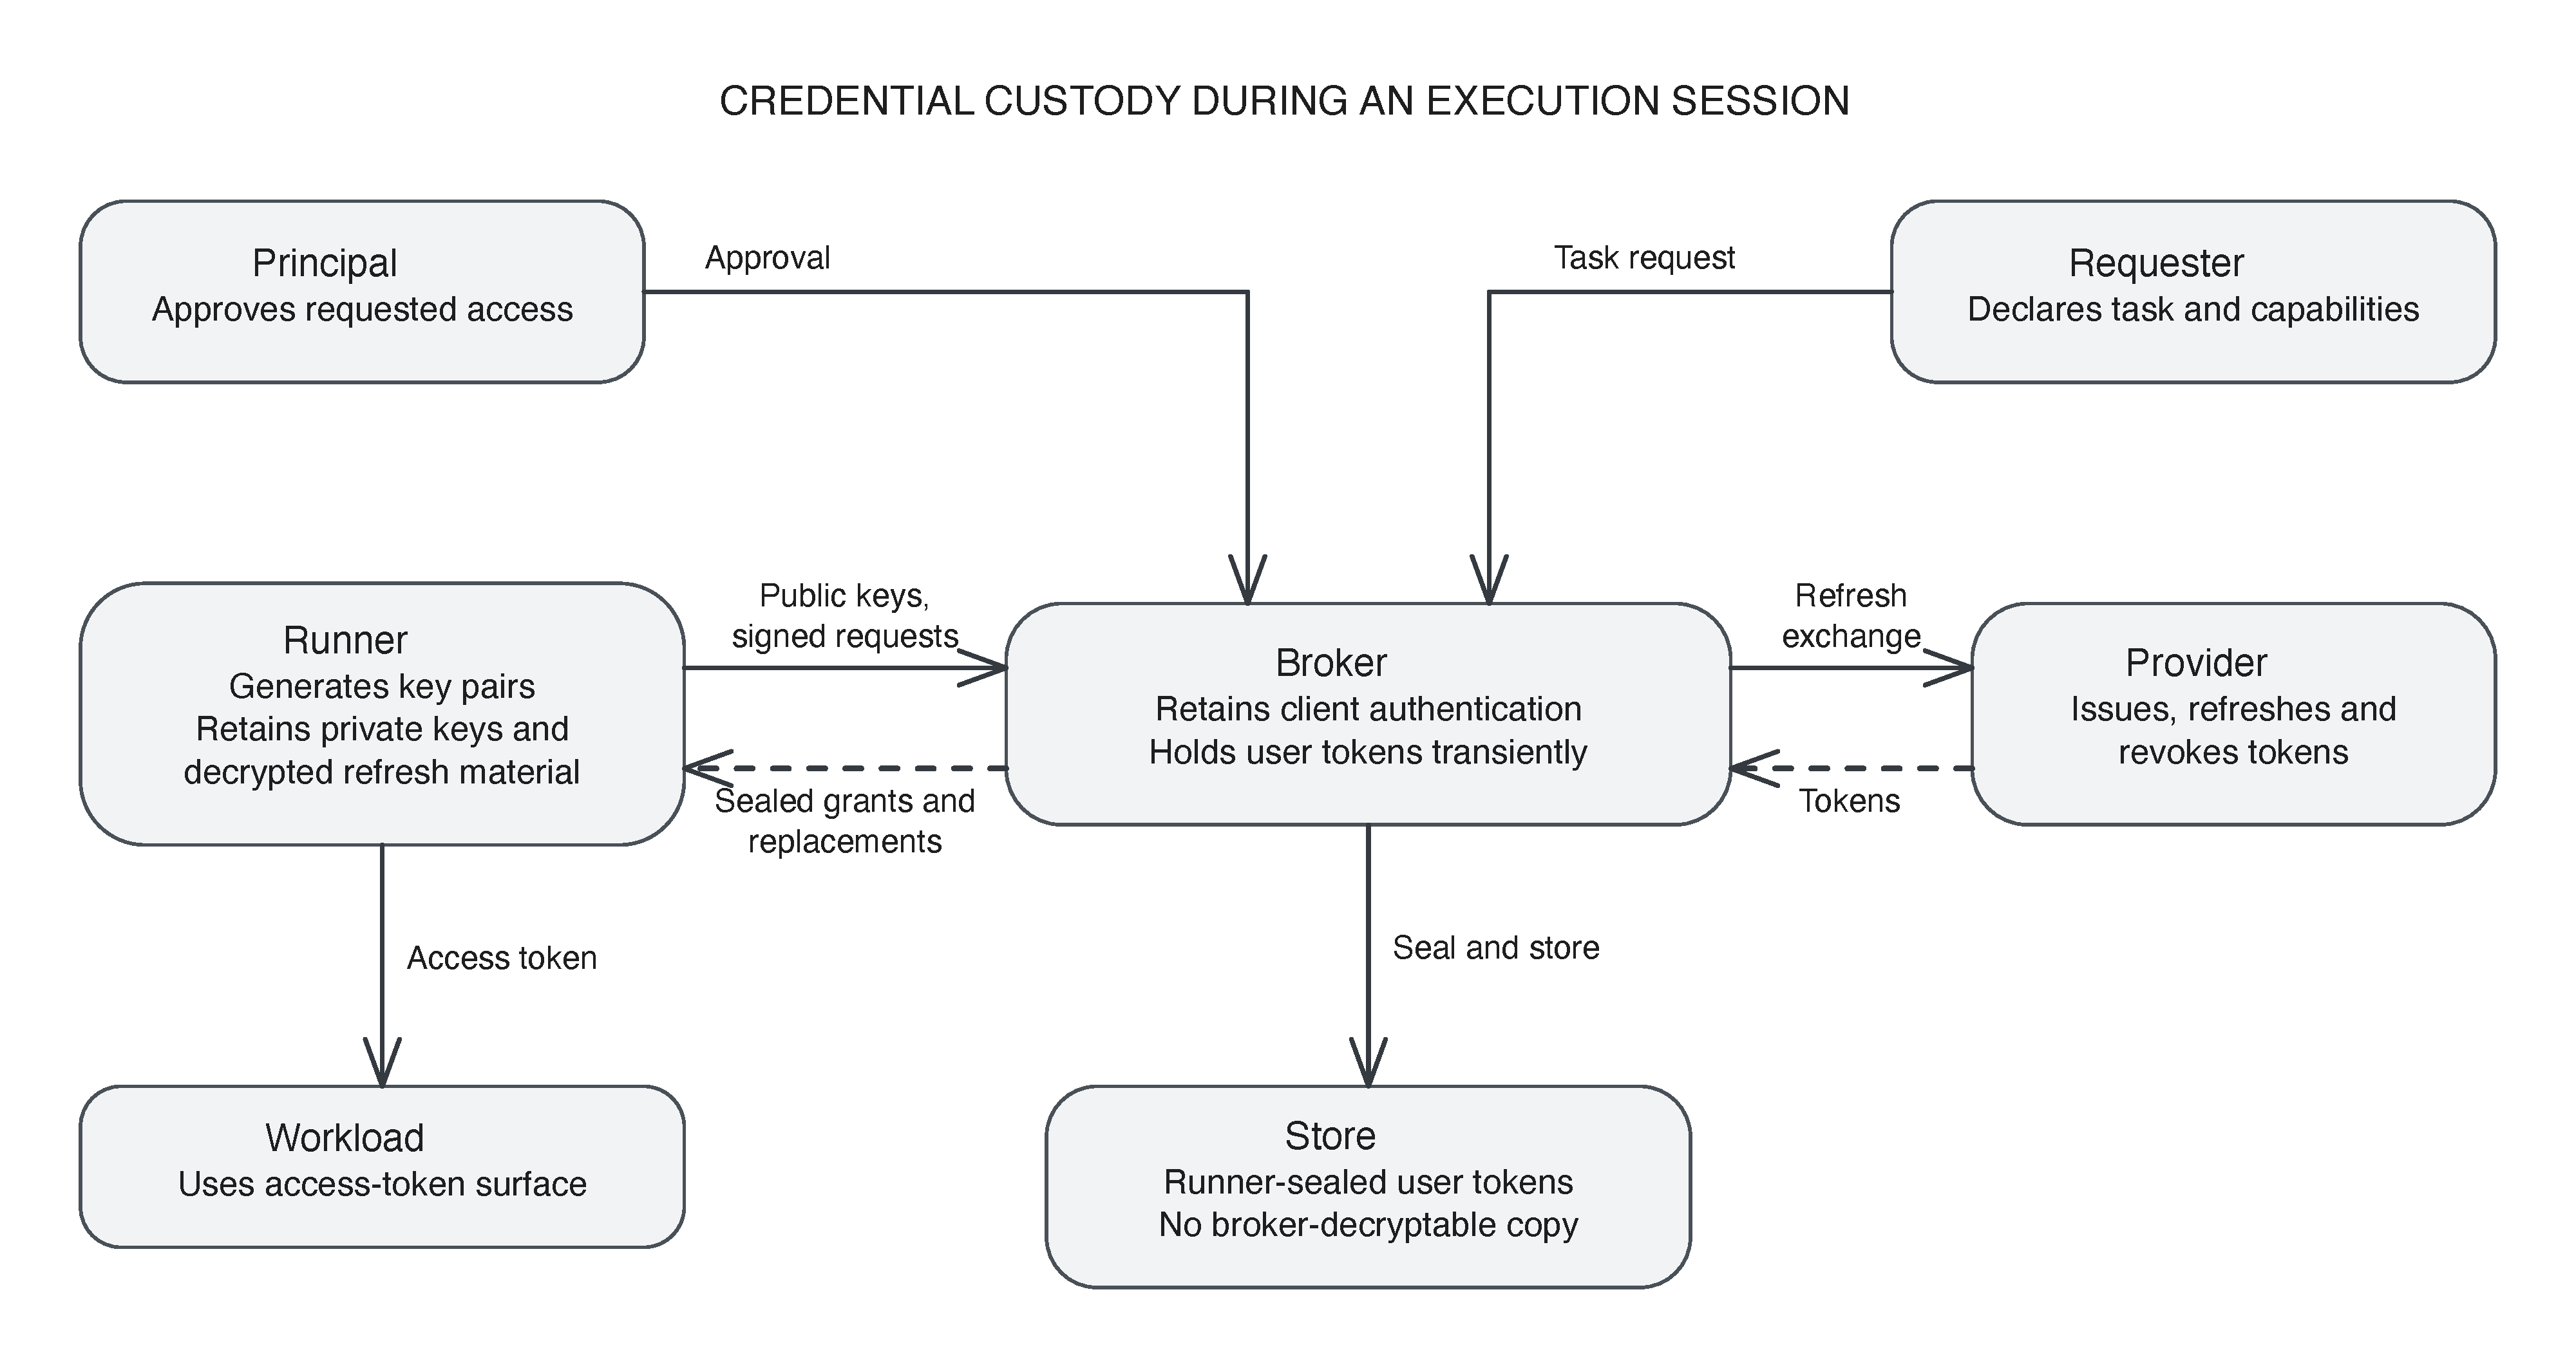
\includegraphics[width=0.9\textwidth]{fig/fig1.pdf}
\caption{Roles and credential custody. The runner retains private keys and decrypted refresh material; the broker retains client authentication and holds user tokens only transiently; the store holds only runner-sealed ciphertext.}
\label{fig:arch}
\end{figure}

\paragraph{Goals.} (G1) No persistent broker-decryptable user token at rest. (G2) The confidential-client secret never reaches the execution environment. (G3) A runner's refresh material is useless without the broker's live cooperation, and vice versa. (G4) Teardown attempts provider revocation. (G5) Child authority is never wider than root, parent and policy authority, including across renewal. (G6) Renewal is possible only for the token lineage issued under the approved grant. (G7) A lost renewal reply is recoverable without a second provider exchange, and an ambiguous provider outcome never leads to a blind retry.

\paragraph{Adversaries considered.} (i) An attacker who obtains a snapshot of the broker's storage. (ii) A model-controlled agent, or content it reads, that induces out-of-scope operations. (iii) Transport faults and duplicated or failed-over callers causing lost, repeated or concurrent renewal requests.

\paragraph{Implementation status.} Sealed delivery, the delivery record, commitment-gated recoverable renewal and cooperative teardown are implemented in an open reference implementation (Section~\ref{sec:impl}). The delegation supervisor, epoch-ordered cancellation and assertion-mediated renewal are designs that are specified and verified as models but have not been built; each is marked where it is described.

\paragraph{Trusted base and non-goals.} The broker, the authoritative control-state store, and (in the supervisor design) the host, container runtime and supervisor are trusted. SCOUT does not defend against a compromised runner during its session (the runner holds a usable access token and refresh token), and it does not shorten provider-token lifetime. Provider support for refresh, rotation and revocation is configuration-dependent; an adapter alone establishes none of them.

\section{Design: Delivery of Sealed Grants}
\label{sec:design}
Figure~\ref{fig:init} shows initial authorization. The runner generates an X25519 encryption key pair and an Ed25519 signing key pair and retains the private keys. A session can be created with the public keys (one-shot) or created first and bound later with the session secret (split creation), which supports tasks that precede their runners. The principal approves the requested capabilities; the broker performs the provider exchange, seals each token to the pinned runner encryption key, and stores only the ciphertext. The runner retrieves the grants with a signing proof and decrypts them in memory.

\begin{figure}[t]
\centering
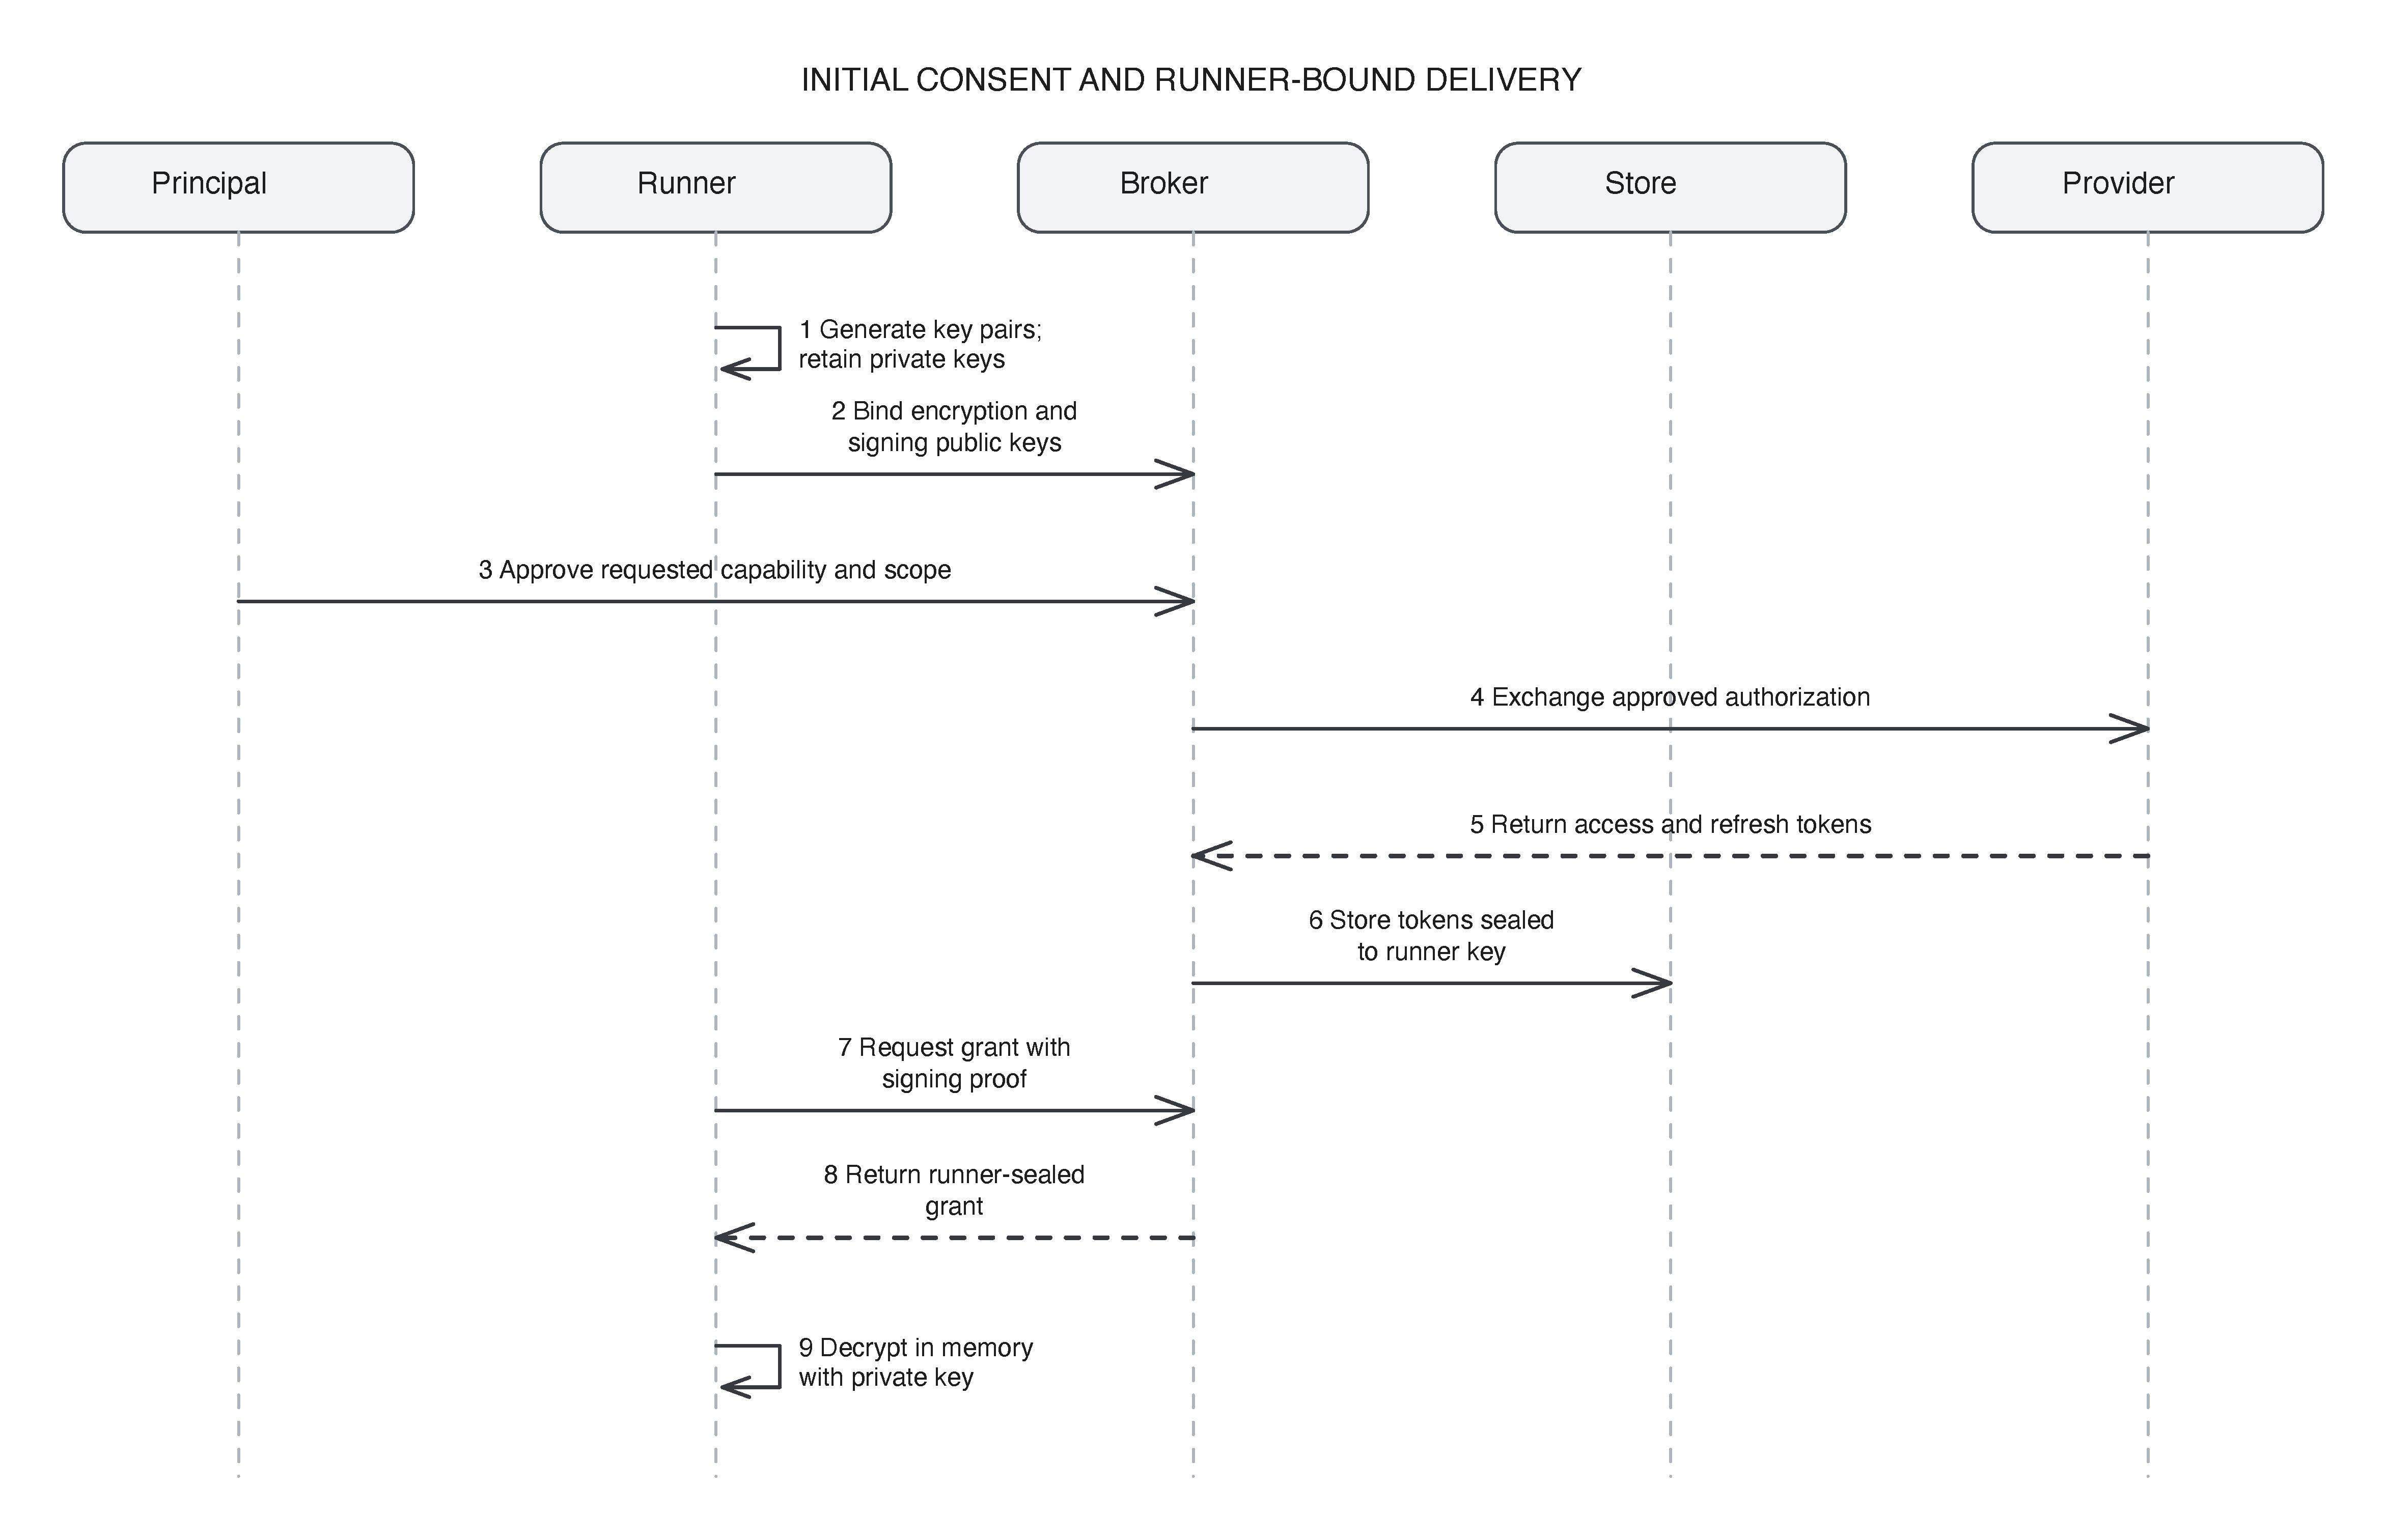
\includegraphics[width=0.92\textwidth]{fig/fig2.pdf}
\caption{Initial consent and runner-bound delivery. The runner binds public keys, the principal approves, the broker stores tokens sealed to the runner key, and the runner decrypts in memory.}
\label{fig:init}
\end{figure}

\paragraph{Sealing.} Each seal generates a fresh ephemeral X25519 sender key pair, derives a shared secret with the runner's public key, derives a 32-byte key with HKDF-SHA256 (domain-separated, with the session and grant identifiers as associated data), and encrypts with AES-256-GCM under a fresh 12-byte IV. A second sealing profile adds the token kind (access or refresh) and the renewal generation to the associated data, so a ciphertext sealed as one kind or in one generation does not open in place of another; a runner that advertised the second profile rejects the first, which prevents downgrade. Equivalent standardized constructions such as HPKE~\cite{rfc9180} are alternatives. \paragraph{Proofs.} The session-bound proof is an Ed25519 signature over canonical JSON of the session identifier and a timestamp, accepted within a bounded window. The store retains only a domain-separated hash of the session secret, compared in constant time.

\paragraph{Delivery record.} The first authorized grant retrieval conditionally commits a delivery record holding the exact sealed response. An identical signed request within its window returns the same response; a different valid request closes delivery and revokes the session. A runner that suffers an uncertain transport outcome keeps its original signed request, because an earlier copy may still be executing, rather than issuing a fresh proof.

\paragraph{Session states.} Sessions move through PENDING, BOUND, AUTHORIZED, ACTIVE, DENIED, REVOKED and EXPIRED; terminal records cannot be mutated and finalization is idempotent.

\section{Design: Session-Gated Renewal with Recoverable Responses}
\label{sec:renewal}
Renewal is where the split-custody property is exercised (Figure~\ref{fig:renew}). The runner decrypts its refresh token and presents it with the current generation receipt and a request-bound proof. The broker verifies the proof against the pinned signing key, accepts only an ACTIVE unexpired session, checks a keyed commitment of the presented token against the approved root, performs the provider refresh using the confidential-client authentication it holds, seals the replacement (and any rotated refresh token) to the same runner key, and returns it. No broker-decryptable copy of the replacement is persisted. A foreign token is rejected before any provider call, even when valid for the same confidential client.

\begin{figure}[t]
\centering
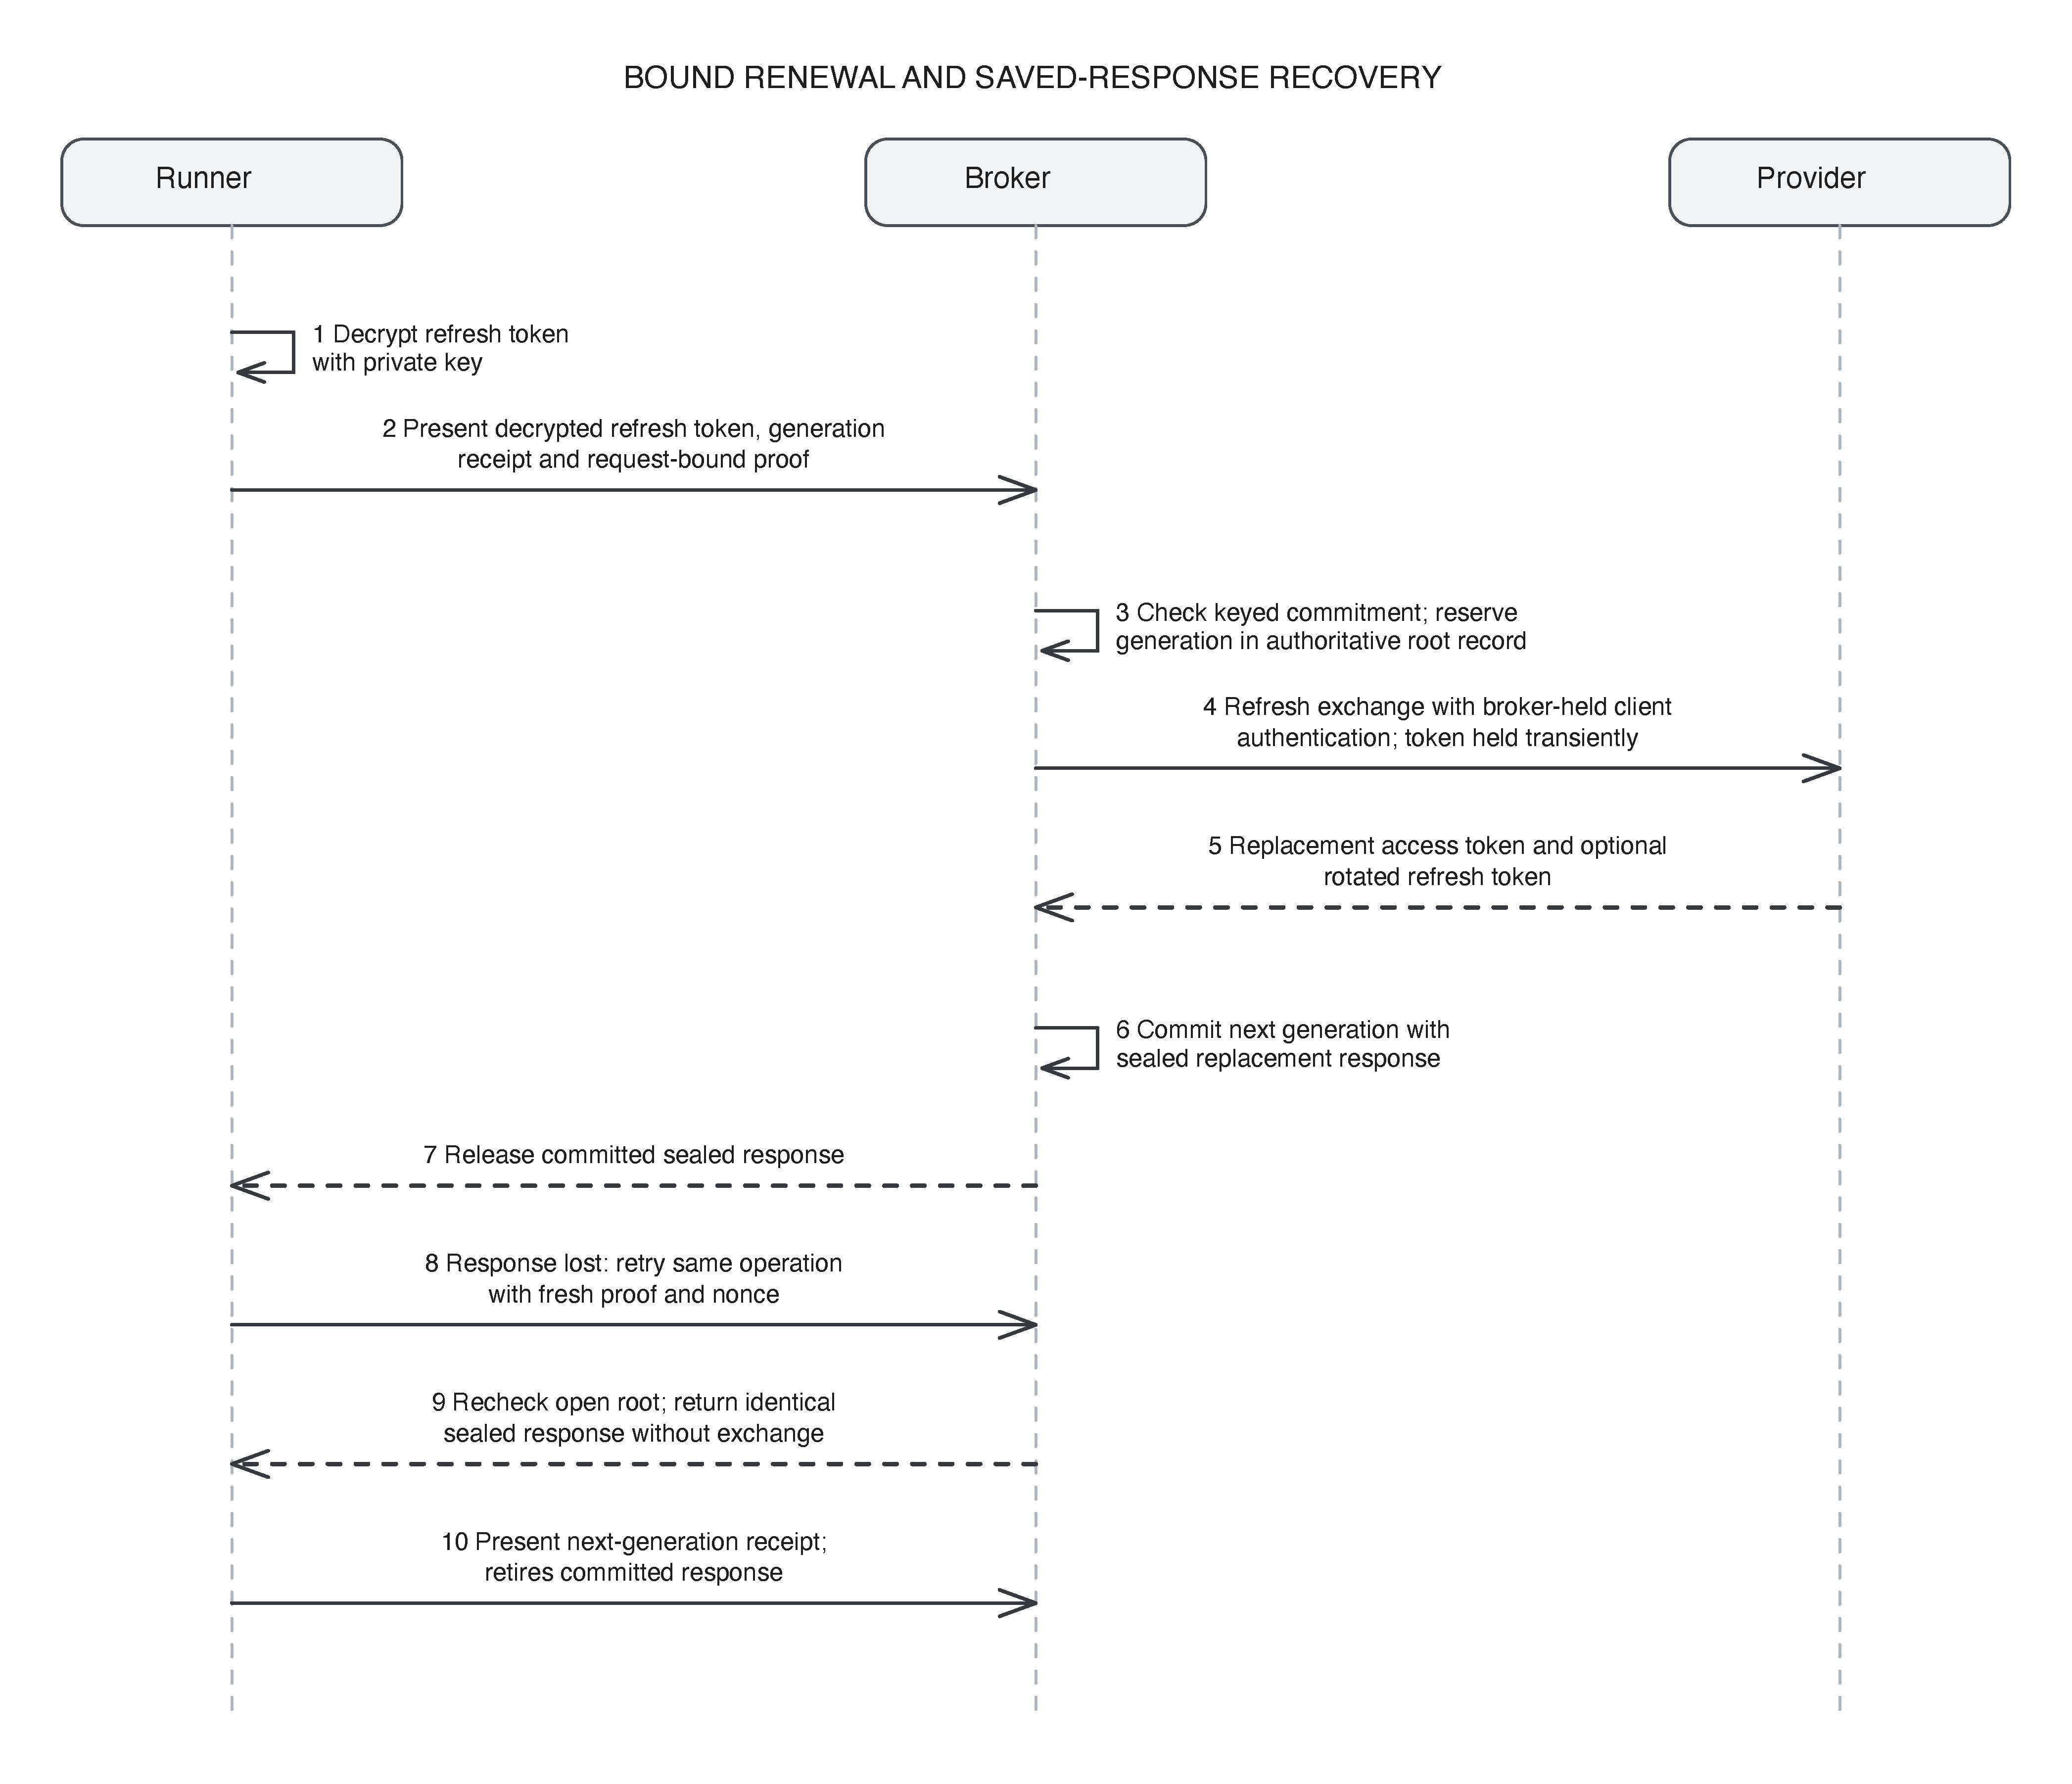
\includegraphics[width=0.78\textwidth]{fig/fig3.pdf}
\caption{Bound renewal and saved-response recovery. The broker reserves a generation, performs one provider exchange, commits the next generation together with the sealed reply, and returns the identical reply on a matching retry.}
\label{fig:renew}
\end{figure}

\paragraph{Two problems the split creates.} \emph{Lost replies.} Providers that rotate refresh tokens invalidate the presented token on use~\cite{rfc9700,ghrefresh}. If the reply carrying the replacement is lost after the provider acted, the caller holds a dead token and no replacement, and only a new approval restores access. An intermediary can save the first response and replay it on retry, as idempotency-key APIs do~\cite{stripe}, but only if it holds the response. A token service that stores only keyed hashes cannot; Ory Hydra records exactly this obstacle and offers a grace period that issues fresh tokens instead~\cite{hydra1831}. A service that stores decryptable tokens can replay, and then a copy of its storage yields usable credentials. \emph{Refresh oracle.} The provider authenticates the \emph{client} at refresh, not the session under which a token was issued. A broker that holds the client credential of a multi-user application and refreshes whatever a runner with a valid proof presents will refresh a token issued under someone else's approval. A valid runner signature shows which runner is asking, not which token it is entitled to renew.

\paragraph{Root-bound receipts and commitments.} At the approved provider exchange the broker records a keyed commitment (e.g., HMAC under a dedicated key distinct from the provider client secret) over a domain separator, root grant, provider/client reference, generation and the exact refresh-token bytes, together with an authenticated receipt binding policy, commitment and runner keys. The broker keeps the nonredeemable commitment and policy but not a decryptable refresh token. The binding is created only at the original consent exchange; the broker never creates a missing binding from a token presented later. On renewal it recomputes the commitment over the presented token and rejects a mismatch \emph{before the client authentication is used and without contacting the provider}.

\paragraph{Reservation and recovery.} Renewal is a small state machine on a conditional-write control record: $\textsf{ACTIVE}(g)\rightarrow\textsf{REFRESHING}(g)\rightarrow\textsf{READY}(g{+}1)\rightarrow\textsf{ACTIVE}(g{+}1)$, with CLOSED and RECOVERY~REQUIRED as additional states (Table~\ref{tab:states}). Reserving generation $g$ atomically selects the single operation allowed to contact the provider. The sealed replacement, the next commitment and the advanced generation are stored in \emph{one} conditional write on the same control record, so the generation advances only if the sealed replacement is stored. Replay needs the response, not a decryptable token, and the stored response is useless to anyone but the runner; this is what removes the obstacle above. If the response is lost, a retry with the same operation identifier returns the same ciphertext and does \emph{not} reconstruct an exchange from a stale token. If the broker crashes after the external exchange but before the durable commit, the orphaned REFRESHING record is treated as ambiguous: the old token is not retried, and recovery needs authoritative reconciliation or fresh consent. A timeout, a provider error or a restart never releases a reserved generation for a second exchange; other capabilities of the session are unaffected. Admission of the next generation implicitly acknowledges and retires the prior result, and the recovery window is fixed at commit time (ten minutes or the root deadline, whichever is earlier). The request proof signs the method and route, the broker authority, the session and capability, the complete receipt, a digest of the refresh token, a stable operation identifier, a timestamp and a fresh nonce.

\begin{table}[t]
\centering
\small
\begin{tabular}{@{}p{0.27\textwidth}p{0.68\textwidth}@{}}
\toprule
Phase & Accepted behaviour \\
\midrule
\textsf{ACTIVE}($g$) & first valid operation identifier reserves renewal \\
\textsf{REFRESHING}($g$) & same-operation polling allowed; competing identifiers cannot start an exchange \\
\textsf{READY}($g{+}1$) & new commitment, receipt and sealed response; same-ID retrieval returns same ciphertext \\
\textsf{ACTIVE}($g{+}1$) & replacement acknowledged; old generation cannot start another exchange \\
CLOSED / RECOVERY REQUIRED & renewal rejected after root closure or ambiguous provider outcome \\
\bottomrule
\end{tabular}
\caption{Renewal phases on the authoritative control record.}
\label{tab:states}
\end{table}

\subsection{Assertion-mediated renewal (designed, not implemented)}
\label{sec:assertion}
Where the provider accepts a signed client assertion~\cite{rfc7523} instead of a shared secret, the broker can stay out of the token path (Figure~\ref{fig:assert}). The runner sends a proof over the session, capability, current receipt, the \emph{digest} of its refresh token, an operation identifier, a timestamp and a nonce; no token is sent. The broker validates as above, compares the digest with a commitment computed over the digest, reserves the generation and issues \emph{one} client assertion for it, with a recorded identifier and a lifetime of at most sixty seconds, sealed to the runner. The runner presents the assertion and the refresh token directly to the provider and then submits a signed completion report carrying the digest of the replacement refresh token, on which the broker advances the commitment and generation. A retry within the assertion lifetime receives the same sealed assertion; a different operation identifier receives none; after an ambiguous outcome no further assertion is issued for that generation.

\begin{figure}[t]
\centering
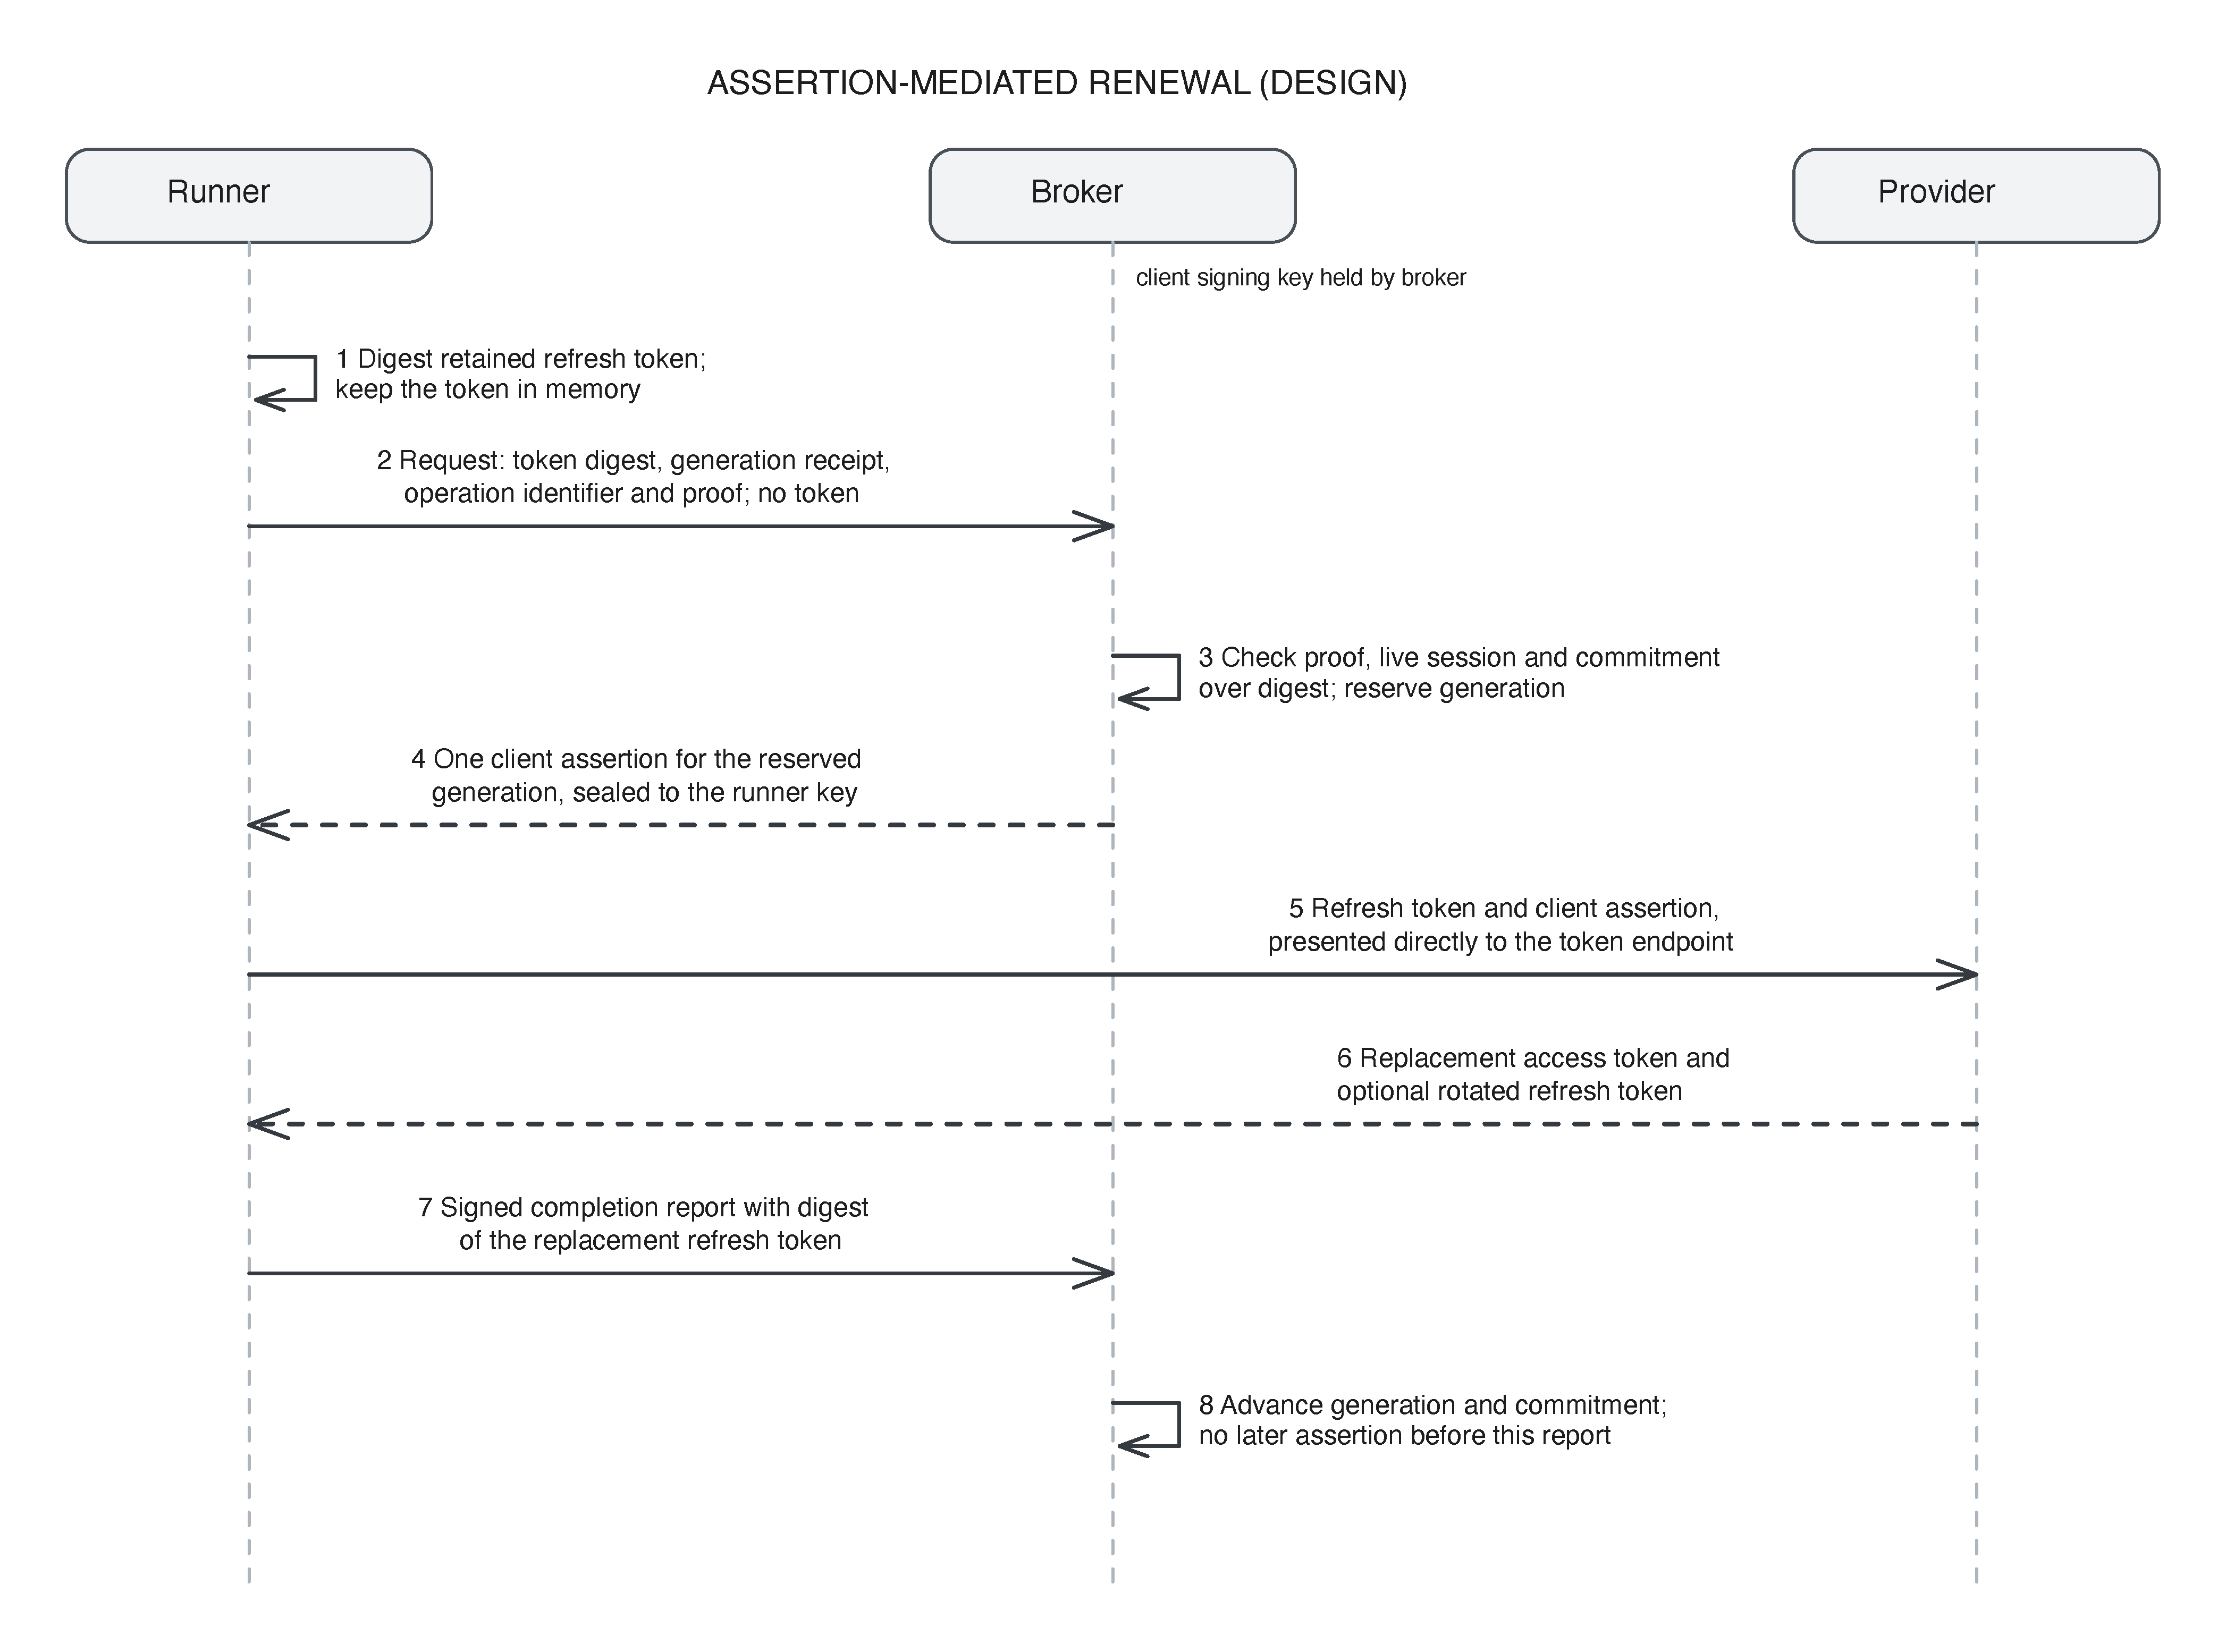
\includegraphics[width=0.78\textwidth]{fig/fig6.pdf}
\caption{Assertion-mediated renewal. The broker issues one client assertion for the reserved generation; the runner performs the provider exchange and reports completion.}
\label{fig:assert}
\end{figure}

No plaintext user token is then present at the broker during renewal, and the client signing key can live in a key-management service from which it cannot be exported. The attestation-based client authentication draft~\cite{attest} also has a backend issue an instance-bound credential, but deliberately permits its reuse; here issuance is tied to one reserved generation. The variant has two weaknesses that we state plainly. The broker cannot verify the reported digest; a false report harms only the reporter, whose next renewal fails the commitment check. And an assertion authenticates the client for \emph{any} refresh token presented with it, so the substitution check is lost unless the provider binds each refresh token to the session, for example by a client identity registered per root grant~\cite{rfc7591} or by sender-constraining the refresh token~\cite{rfc9449}. There is also no sealed reply to replay, because the provider answers the runner directly.

\section{Design: Cooperative Teardown}
\label{sec:teardown}
With only runner-sealed tokens retained, the broker cannot revoke on its own, so teardown is cooperative (Figure~\ref{fig:teardown}). The runner supplies its held access tokens (and, where the provider supports it, refresh tokens) with a signing proof; the broker first checks that each submitted token was delivered in a grant of that session (by a keyed digest recorded at sealing), so a runner cannot use the broker's client credential to revoke arbitrary tokens of the shared client, then attempts each provider-specific revocation~\cite{rfc7009} with the client authentication it holds and reports a per-capability outcome: \emph{acknowledged}, \emph{unsupported}, \emph{failed} or \emph{unknown}. Only a provider acknowledgement counts as revoked. A separately authenticated finalization then closes the shared delivery-and-renewal record and deletes session, consent-index and grant records. Revocation runs first so the broker can still verify the runner key; failures do not block local deletion. Closure blocks new delivery, renewal admission and renewal completion, removes bindings, commitments and saved ciphertext, and leaves a closed marker beyond the session deadline. On the runner side, a command-line wrapper polls signed session status and runs the workload in its own process group; on a terminal session, on repeated failed polls, or on local expiry it terminates the group (a termination signal, then a kill signal after a grace period) and runs teardown. A failed poll is treated as fail-closed.

\begin{figure}[t]
\centering
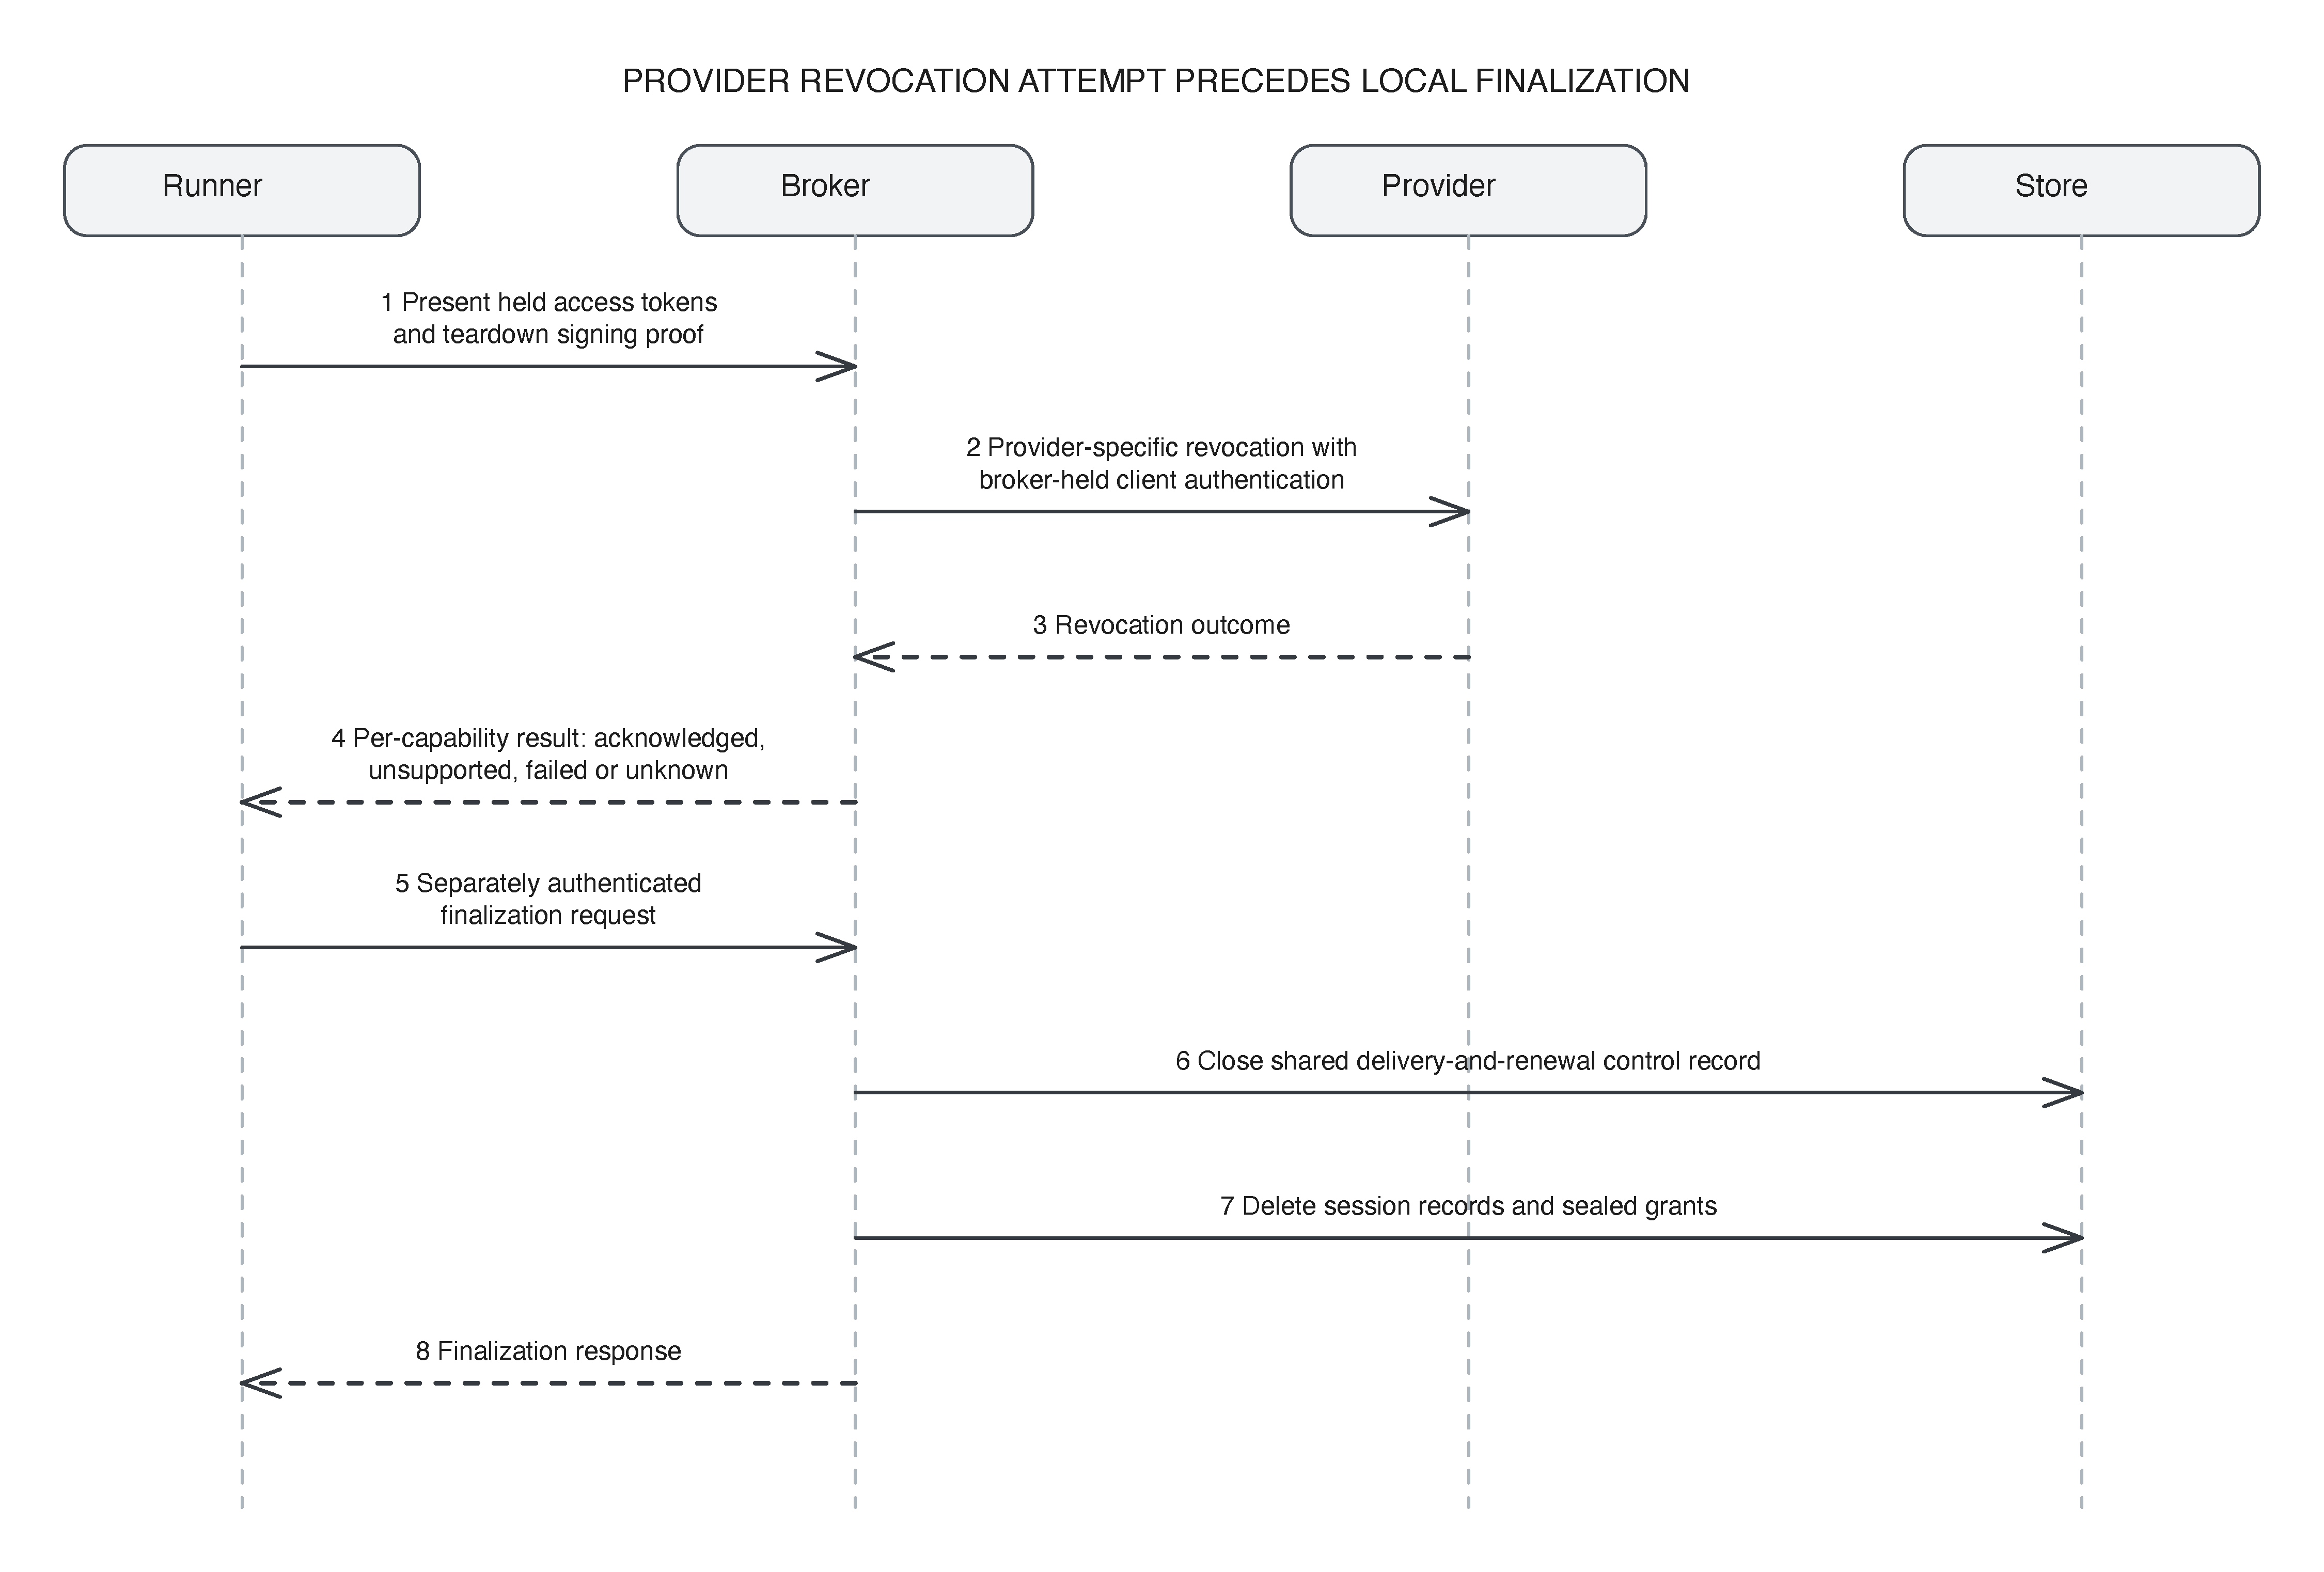
\includegraphics[width=0.85\textwidth]{fig/fig4.pdf}
\caption{Provider revocation is attempted before local finalization.}
\label{fig:teardown}
\end{figure}

We stress the limits: where a runner is unavailable or the provider lacks revocation, residual access is bounded by provider token lifetimes (including any outstanding refresh token, which may far exceed the access-token lifetime), and a finalized response certifies only local cleanup. Revoking an access token alone may leave a refresh token valid.

\section{Design: Supervised Delegation}
\label{sec:supervisor}
Split custody protects tokens at rest, but a workload that is handed a usable access token can still misuse it, and a broad provider scope does not narrow itself for a child agent. In an optional design (Figure~\ref{fig:super}) an \textbf{isolated supervisor} plays the runner role for the root grant: it owns the encryption/signing private keys and the root refresh family, and every provider request for that family passes through its adapter, which injects credentials only after authorization. Model-controlled parent and child agents hold \emph{handles}, not credentials. Isolation requires an OS, container, VM or hardware-backed boundary that prevents model-controlled processes from reading supervisor memory or bypassing mediation.

\paragraph{Authority.} An authorization record captures the root grant, principal, approved constraints, refreshability, epoch and generation. Effective child authority is the intersection of human-approved root authority, effective parent authority, the requested child constraints and supervisor policy, expressed as resource/operation/argument tuples so that independent resource and verb lists cannot be recombined. Child expiry cannot exceed parent or root expiry, and a delegation budget bounds further delegation. Task text supplies correlation, not permission.

\paragraph{Per-operation check.} For each proposed operation the supervisor (1) authenticates the child key, handle and request proof; (2) reads authoritative root and ancestor state and rejects expired, revoked or superseded authority; (3) canonicalizes method, target, resource, operation and security-relevant arguments, rejecting ambiguous mappings; (4) evaluates the exact tuple against effective authority and the current epoch and atomically records a one-time reservation; (5) renews the root credential if needed, revalidates, and sends the request with the credential injected inside the boundary; and (6) records a sanitized decision without credential values.

\begin{figure}[t]
\centering
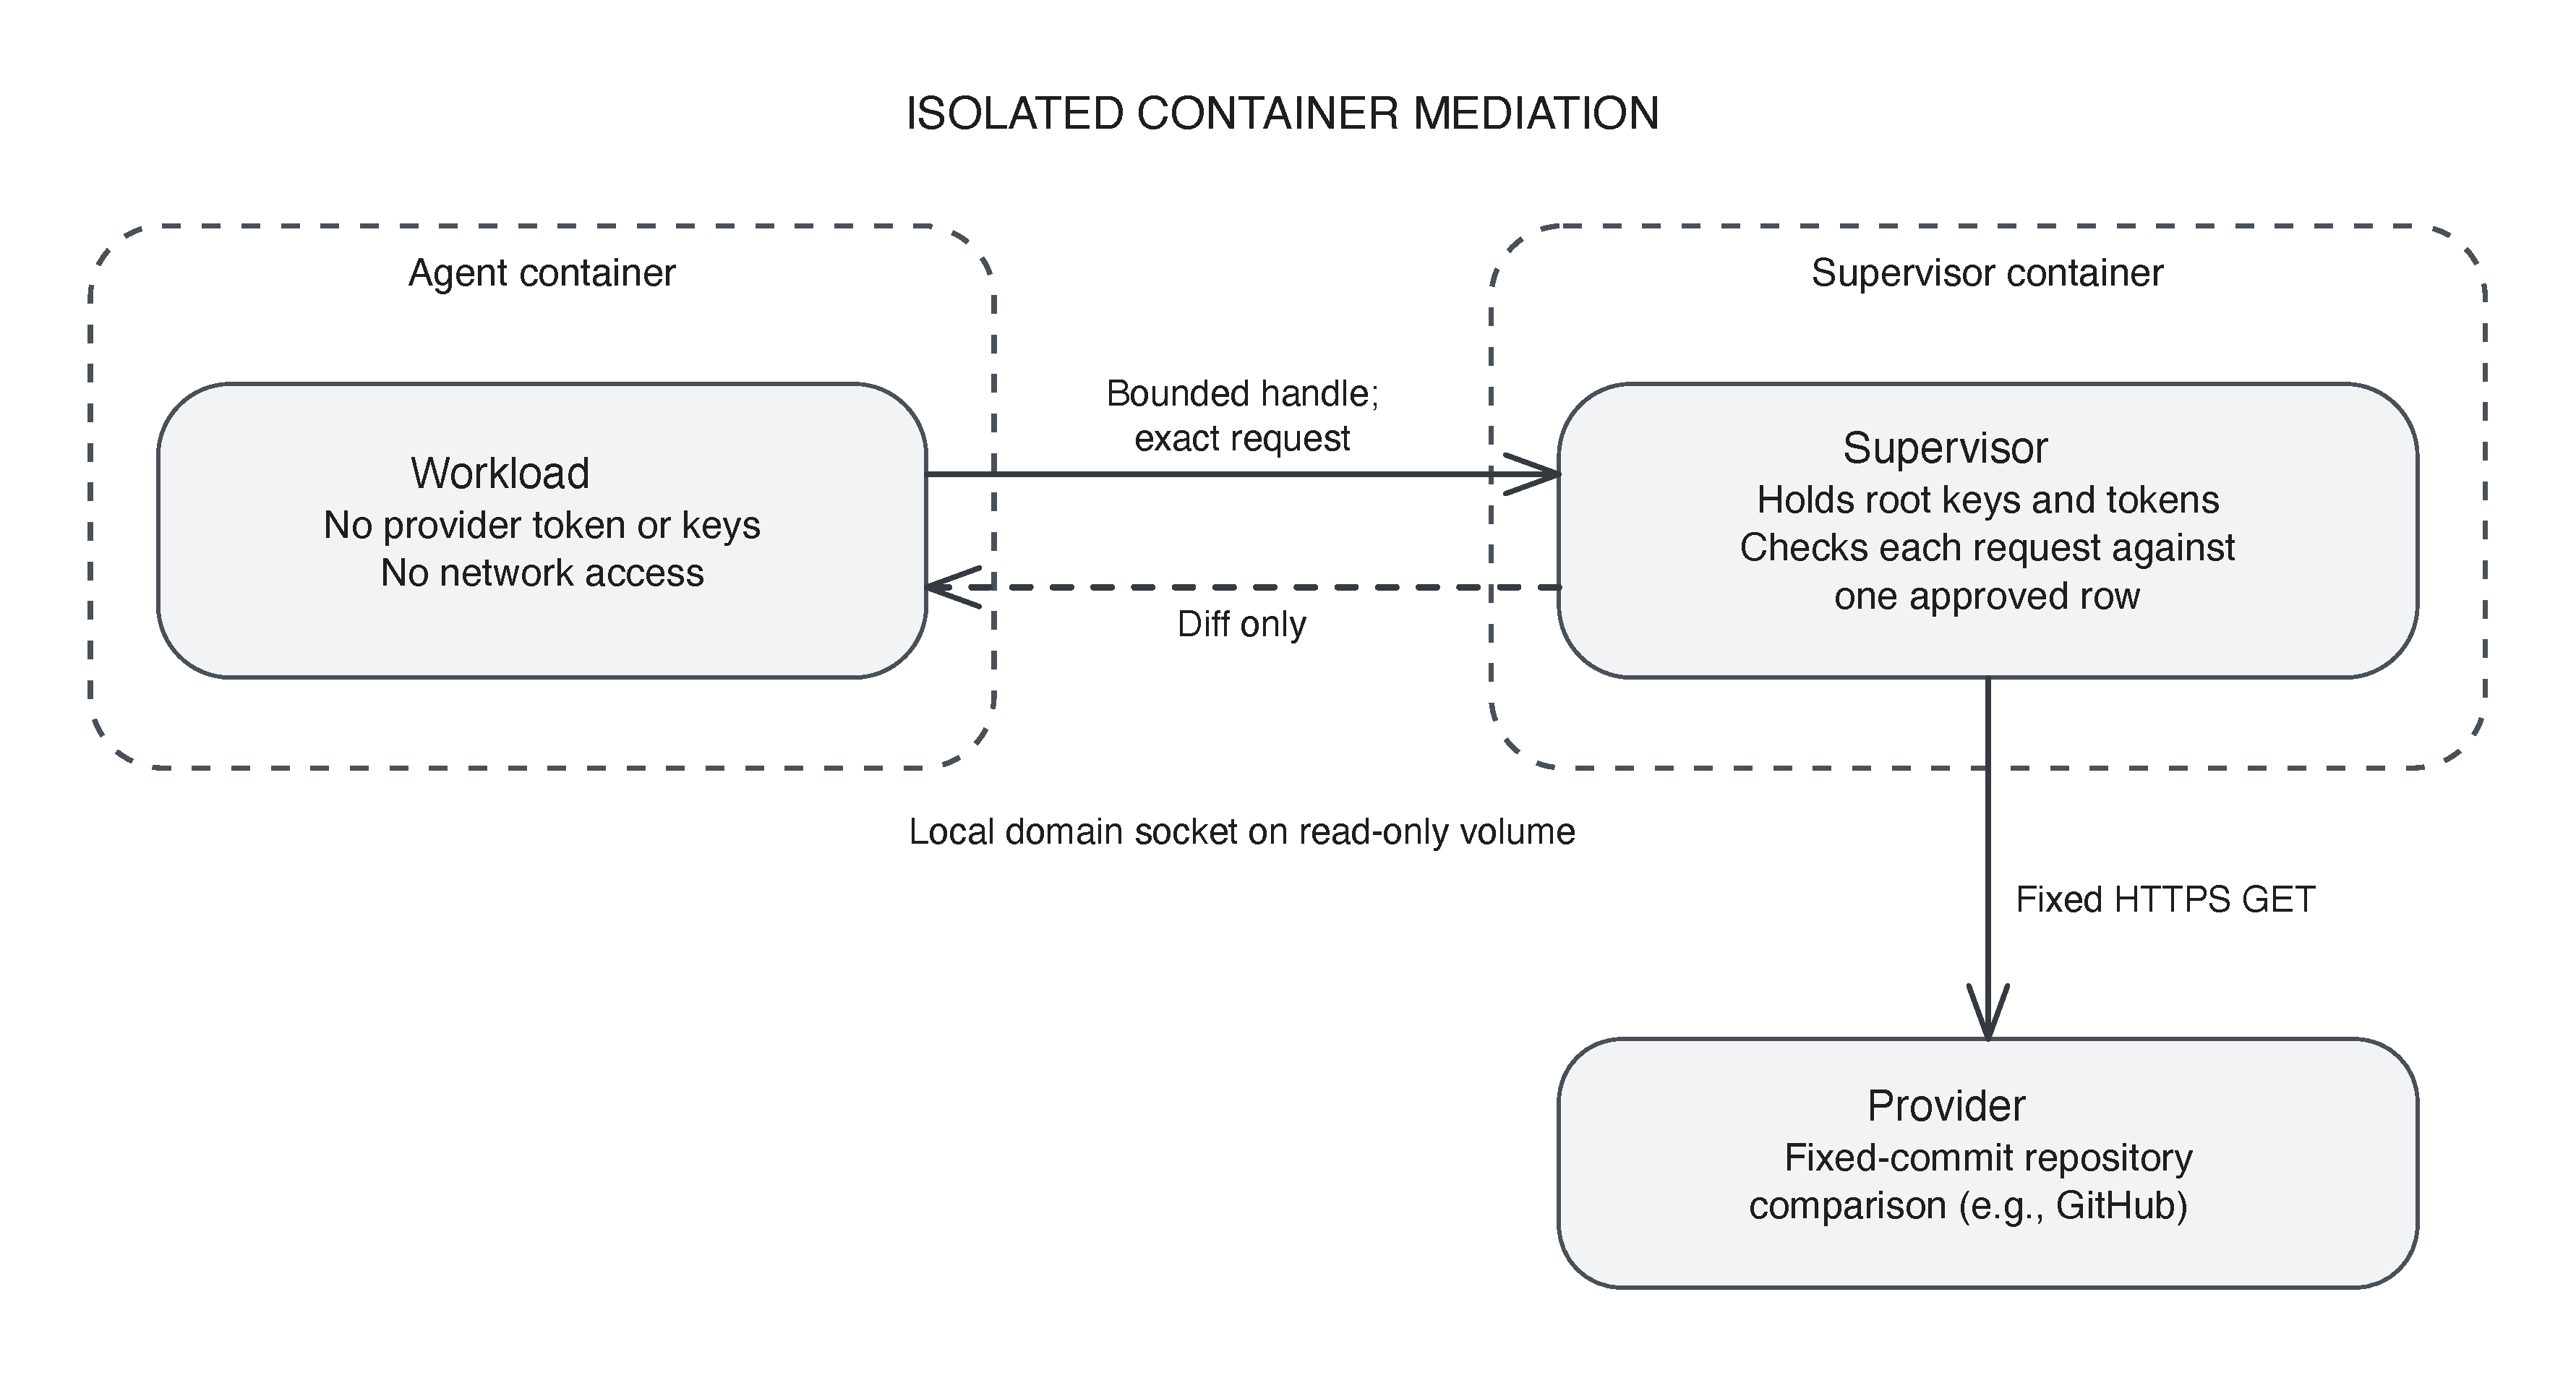
\includegraphics[width=0.78\textwidth]{fig/fig5a.pdf}\\[4pt]
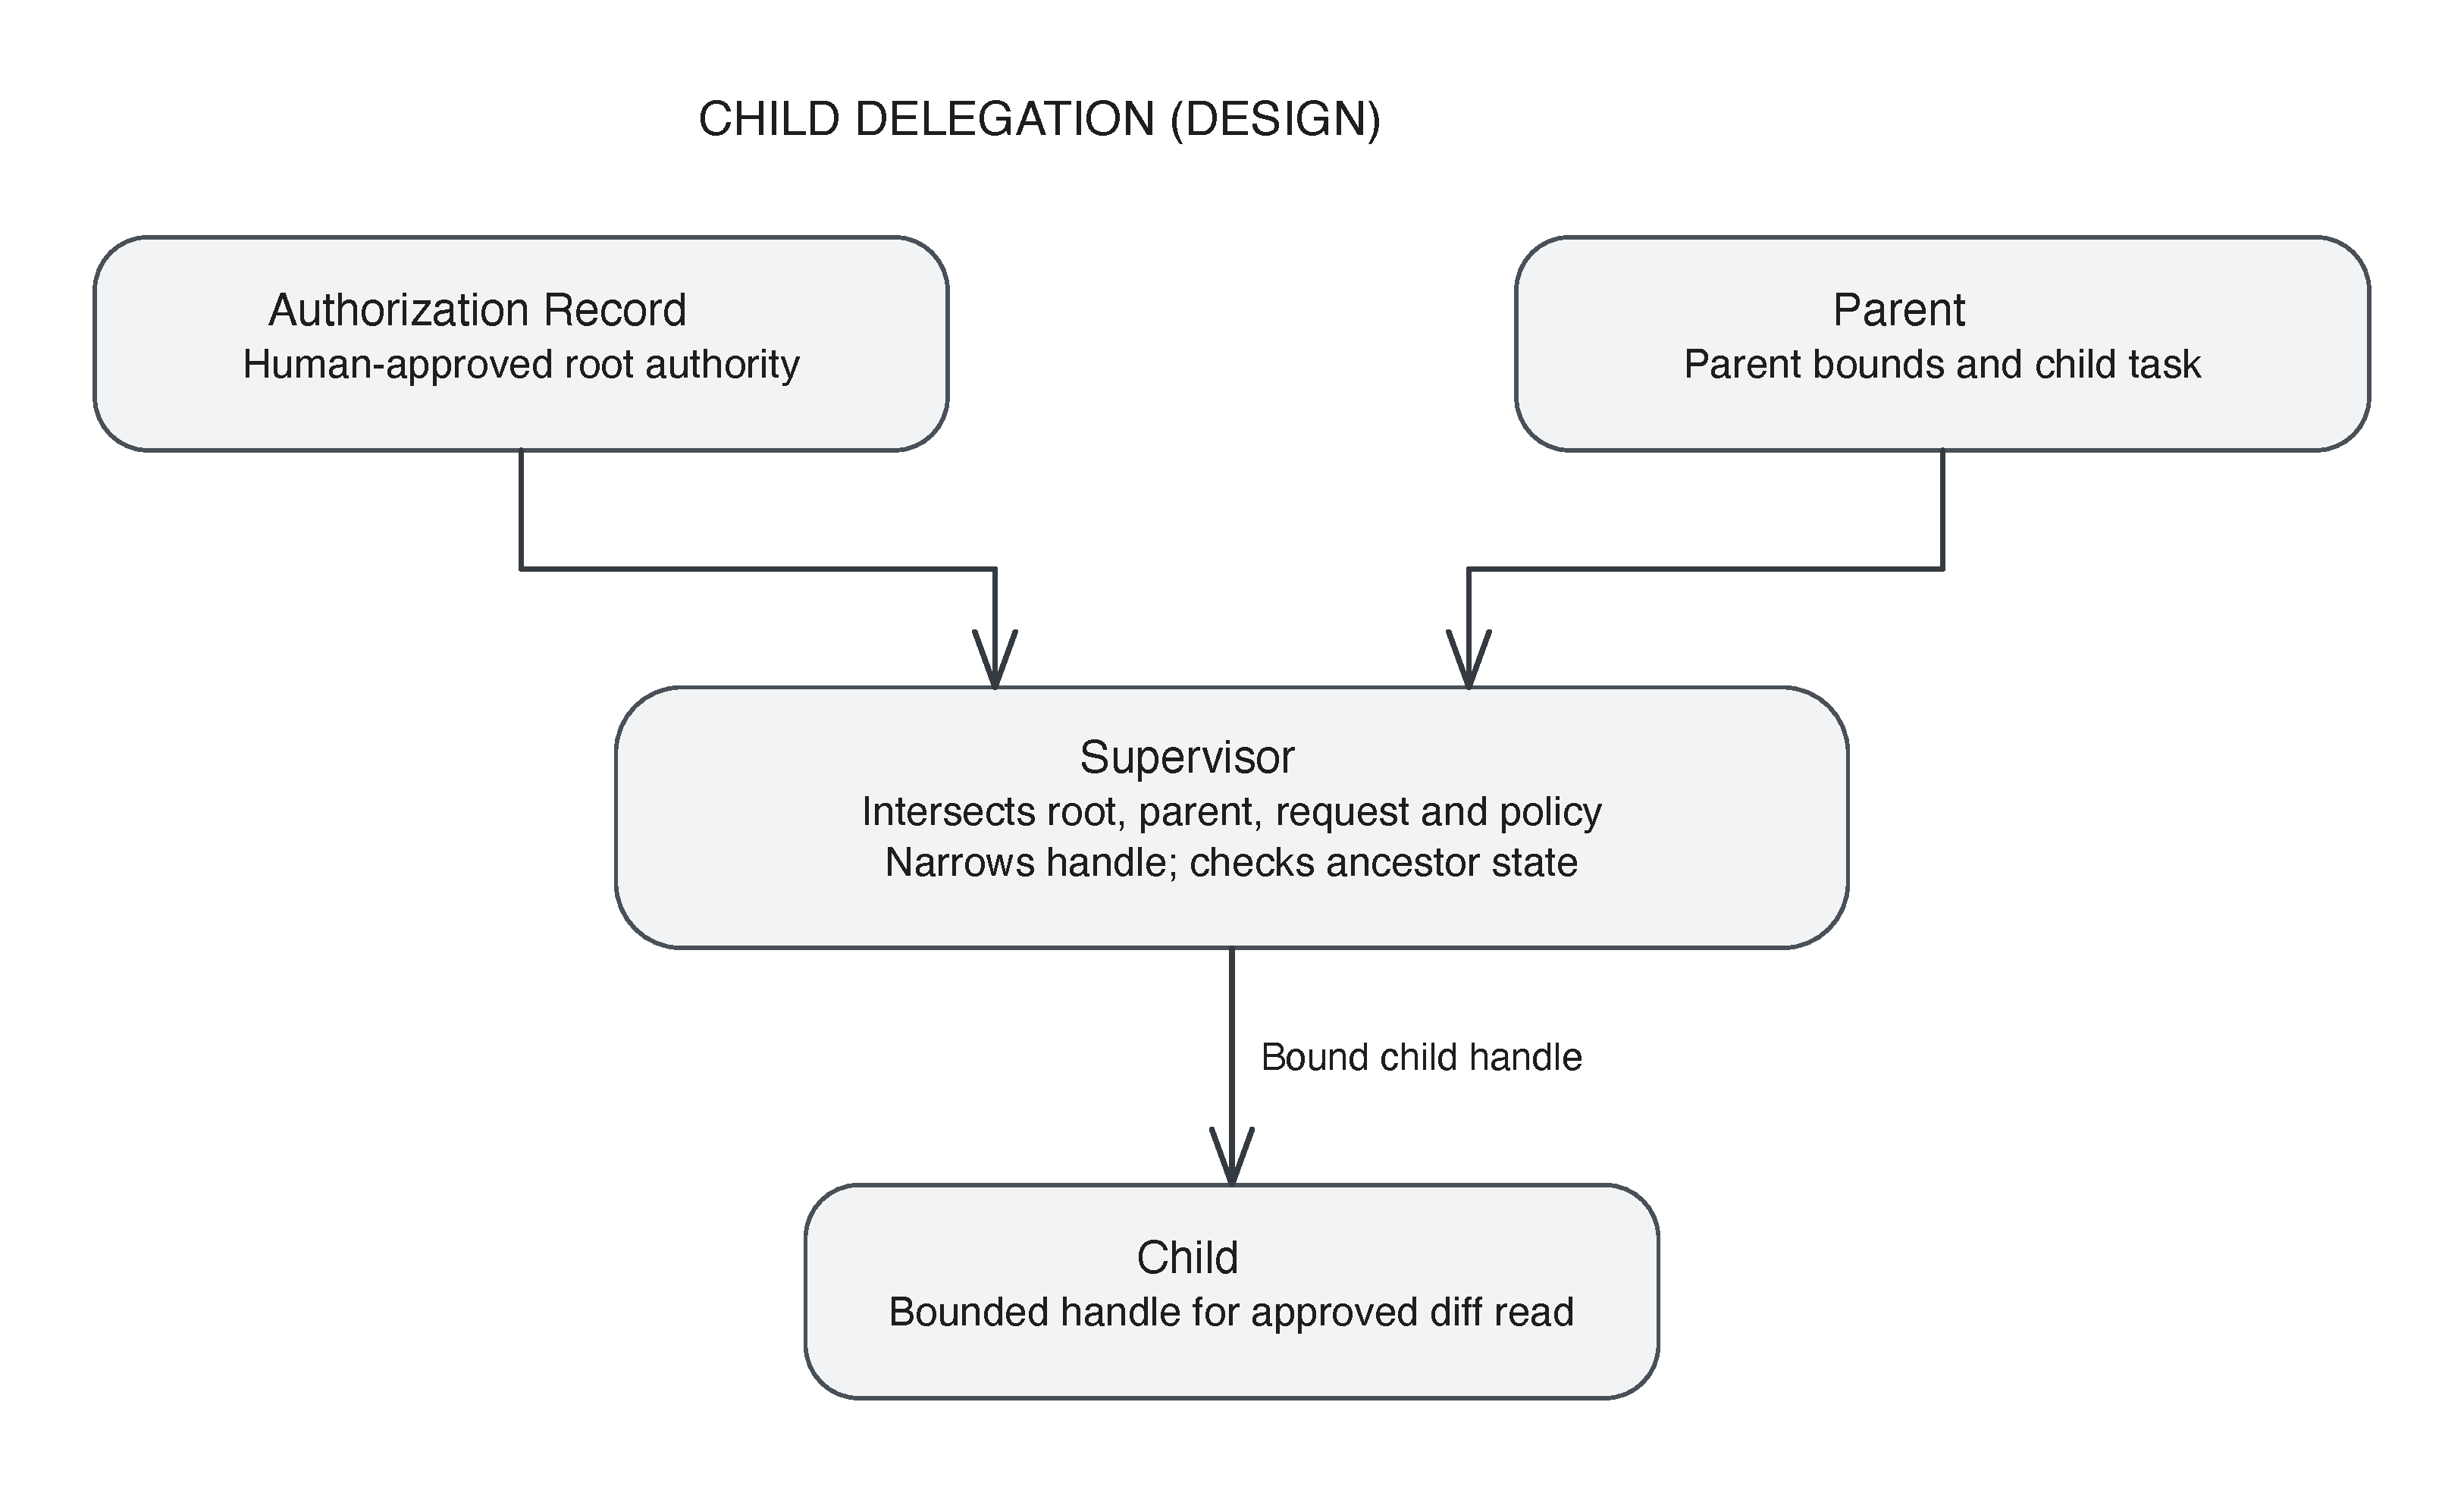
\includegraphics[width=0.78\textwidth]{fig/fig5b.pdf}
\caption{(Top) Container-isolated mediation of a read-only repository diff: the workload has no provider token, keys or network, and the supervisor admits a request only if it matches one approved row. (Bottom) The supervisor narrows child authority to the intersection of root, parent, request and policy.}
\label{fig:super}
\end{figure}

\paragraph{Example.} A principal approves a coding task for repository A. A parent requests a child reviewer; the supervisor issues a handle bound to the child's identity and key, the repository, an immutable diff identifier, a read-diff operation and a deadline no later than the parent's. If content inside the diff induces the model to propose a push to repository B, the supervisor denies it: the check constrains the operation independently of the model's proposal, and the child never holds the root refresh token. In the simplest deployment of this design the workload runs in a separate container with its own process namespace and no network, with only a Unix socket and bounded handle handed in.

\paragraph{Shared renewal.} Several children may need the root credential replaced at once. The generation reservation of Section~\ref{sec:renewal} ensures the shared family is rotated once; waiting children are served with the resulting credential while keeping their own distinct permissions, and cancellation serializes against the same authoritative epoch so new reservations and response releases fail after closure.

\section{Verification}
\label{sec:eval}
We checked the protocol with six complementary methods: SMT, Lean, TLA\textsuperscript{+}, a custody closure and ProVerif on models (this section), and Kani on the code of the reference implementation (Section~\ref{sec:impl}). All scripts, models, code and outputs are public at \url{https://github.com/Algiras/scout-proofs} (see the reproducibility note). Section~\ref{sec:evallimits} states what remains unproven.

\subsection{Inductive invariants, discharged by an SMT solver}
\label{sec:smt}
Each part of the protocol is written as a transition system over the durable control record, the broker's volatile state, and ghost variables that record what the specification cares about (for example, how many provider exchanges were performed for a generation). For a set of safety properties $S$ we give an invariant $\mathit{Inv} \Rightarrow S$ and ask Z3~\cite{z3} to show that the three standard obligations are unsatisfiable when negated:
\[
\mathit{Init} \Rightarrow \mathit{Inv}, \qquad \mathit{Inv} \wedge T \Rightarrow \mathit{Inv}' \ \text{ for every transition } T .
\]
The formulas are quantifier-free over linear integer arithmetic and booleans. Generations, operation identifiers, tokens, clocks and epochs are unbounded integers, and per-generation properties are stated for an arbitrary symbolic generation $g_0$, so each result holds for \emph{any} number of generations, retries, crashes and concurrent callers rather than within a bound. Table~\ref{tab:smt} lists the properties; all 41 obligations are proved, in a few seconds in total.

\begin{table}[t]
\centering
\small
\begin{tabular}{@{}p{0.19\textwidth}p{0.62\textwidth}r@{}}
\toprule
Model & Properties proved for every reachable state & Obl. \\
\midrule
Session lifecycle & F1 tokens are minted only for a pinned runner key; F2 grants are sealed to the pinned key; F3 one principal per session; F4 terminal states are absorbing & 8 \\
Delivery record & D1 every released response is the first one; D2 nothing is released after revocation & 5 \\
Renewal record & S1 at most one provider exchange per generation; S2 the client authentication is used only with the root's current token; S3 every delivery for a generation is the committed ciphertext; S4 no reply is released after closure; S5 a committed reply stays retrievable until retired, lapsed or closed & 8 \\
Assertion-mediated renewal & M1 at most one client assertion per generation; M2 assertions are issued only for a live, open session whose committed digest matches the held token; M3 no assertion is returned after expiry or closure & 8 \\
Teardown and closure & T1 the client authentication revokes only tokens delivered in that session; T2 ``revoked'' is reported only on provider acknowledgement; T3 no delivery, renewal admission or completion after closure; T4 records and the runner key are deleted only after closure; T5 closure leaves no bindings or saved ciphertext; T6 revocation requests are verified against a retained runner key & 7 \\
Authorization epoch & A1 no reservation after closure or expiry; A2 no dispatch under a superseded epoch & 5 \\
\bottomrule
\end{tabular}
\caption{Inductive-invariant proofs. ``Obl.''\ is the number of proof obligations (initiation plus one per transition).}
\label{tab:smt}
\end{table}

The renewal model has seven transitions: \textsf{Reserve} (admission, guarded by the commitment check), \textsf{Exchange} (the provider call, after which the provider may or may not have rotated the token), \textsf{Commit} (the single conditional write), \textsf{Replay}, \textsf{Crash} (volatile state lost at any point, reservation kept), \textsf{Close} and \textsf{Expire}. S1 and S2 together say that the broker never presents a possibly-consumed token: after a crash between \textsf{Exchange} and \textsf{Commit} no transition is enabled that would call the provider again for that generation. S3 and S5 are the recovery guarantee: once a generation is committed, the identical ciphertext is what any retry receives.

The assertion-mediated model covers the completion report that the broker cannot verify: after a false report the committed digest no longer matches the token the runner holds, and by M2 no further assertion is issued for it. The teardown model covers the ordering of Section~\ref{sec:teardown}: revocation while the runner key is still retained, then closure, then deletion.

The delegation rule is proved as one inductive step over 64-bit permission masks: if the parent's authority is within the root's, the child computed as $\mathit{root} \cap \mathit{parent} \cap \mathit{requested} \cap \mathit{policy}$ is within both, and its expiry and delegation budget do not exceed the parent's. By induction this holds for a lineage of any depth.

\paragraph{Broken variants.} A proof is only as good as the model, so each property is paired with a deliberately defective variant, and bounded model checking from the initial state must return a concrete violating trace (a failed induction step alone would not show reachability). All 26 variants are caught (Table~\ref{tab:neg}), as is the broken delegation rule that takes a union with the request.

\begin{table}[t]
\centering
\small
\begin{tabular}{@{}p{0.36\textwidth}lp{0.47\textwidth}@{}}
\toprule
Defect & Violates & Shortest trace \\
\midrule
Consent allowed before binding & F1 & Consent \\
Rebinding after consent & F2 & Bind, Consent, Bind \\
No principal lock & F3 & Bind, Consent, Consent \\
Expired session reopened & F4 & Expire, Reopen \\
A new proof gets a new response & D1 & Fetch, FetchOther \\
Session write resets delivery & D1 & Fetch, SessionWrite, Fetch \\
Refetch ignores revocation & D2 & Fetch, Revoke, Refetch \\
Reservation released on timeout & S1 & Reserve, Exchange, Crash, Reserve, Exchange \\
No commitment check & S2 & Reserve, Exchange \\
Competing operation admitted & S1 & Reserve, Exchange, Reserve, Exchange \\
Generation advances without stored reply & S5 & Reserve, Exchange, Commit \\
Reply resealed on retry & S3 & Reserve, Exchange, Commit, Replay \\
Reply released after closure & S4 & Reserve, Exchange, Commit, Close, Replay \\
Fresh assertion on retry & M1 & ReserveIssue, Retry \\
Reservation released when assertion expires & M1 & ReserveIssue, AssertionExpires, ReserveIssue \\
Assertion issued without digest check & M2 & ReserveIssue, Complete, ReserveIssue \\
Assertion issued after closure & M2 & Close, ReserveIssue \\
Assertion returned after expiry & M3 & ReserveIssue, AssertionExpires, Retry \\
Revoke any submitted token & T1 & Revoke \\
Error or timeout reported as revoked & T2 & Revoke \\
Renewal completes after closure & T3 & Close, RenewCommit \\
Delete before close & T4 & Delete \\
Closure keeps ciphertext & T5 & Close \\
Revoke after key deleted & T6 & Delete, Revoke \\
Check, then reserve (not atomic) & A1 & Check, Cancel, Reserve \\
Dispatch without revalidation & A2 & Reserve, Cancel, Dispatch \\
\bottomrule
\end{tabular}
\caption{Deliberately broken variants and the counterexamples found by bounded model checking.}
\label{tab:neg}
\end{table}

\subsection{The same obligations, checked by the Lean kernel}
\label{sec:lean}
An SMT result rests on trusting the solver. To remove that dependency, the six transition systems are exported mechanically, from the same definitions, to Lean~4~\cite{lean4}. Each proof obligation of Table~\ref{tab:smt} becomes a theorem over unbounded integers and booleans, with the post-state substituted into the invariant, and each safety property becomes a theorem that it follows from the invariant: 63 theorems in total (41 obligations and 22 safety properties). All are accepted by the Lean kernel (version 4.36.0) and depend only on Lean's three standard axioms (\texttt{propext}, \texttt{Classical.choice}, \texttt{Quot.sound}); no theorem uses \texttt{sorry}. As a negative control, the same export applied to the 26 broken variants yields theorems that Lean rejects in every case. The two tools therefore agree on every obligation, and the unbounded results of this section do not rest on Z3 alone.

\subsection{The same systems in \texorpdfstring{TLA\textsuperscript{+}}{TLA+}, model-checked by TLC}
\label{sec:tla}
The same export also produces TLA\textsuperscript{+} modules~\cite{tla}, one per transition system, with each safety property as an invariant. TLC explores every reachable state within finite bounds: parameters range over two values (four for the provider's revocation answer), the symbolic generation and the expiry over three, and generation, clock and epoch counters are cut off at three. All six models pass (Table~\ref{tab:tlc}). Each of the 26 broken variants is exported as its own module, and TLC reports its invariant violated in every case. TLC adds nothing to the unbounded results above; its value is that TLA\textsuperscript{+} is the notation most engineers who build such services already read, and that it is a third independent implementation agreeing on every model and every counterexample. One bound we first chose was wrong: it also capped the session-state variable, which hid the terminal states and with them one of the defects. The negative control exposed this, which is the reason every property is paired with one.

\begin{table}[t]
\centering
\small
\begin{tabular}{@{}lrr@{}}
\toprule
Model & Distinct states & Broken variants violated \\
\midrule
Session lifecycle & 280 & 4 of 4 \\
Delivery record & 24 & 3 of 3 \\
Renewal record & 23,616 & 6 of 6 \\
Assertion-mediated renewal & 2,352 & 5 of 5 \\
Teardown and closure & 8 & 6 of 6 \\
Authorization epoch & 80 & 2 of 2 \\
\bottomrule
\end{tabular}
\caption{TLC results on the exported TLA\textsuperscript{+} modules, within the stated bounds.}
\label{tab:tlc}
\end{table}

\subsection{Custody closure}
\label{sec:custody}
Goals G1--G3 are statements about who can derive what. We encode the custody rules as Horn clauses under perfect cryptography (a sealed token opens only with the runner decryption key; a provider that authenticates the client refreshes only with both the refresh token and the client authentication; the broker renews only for a live session, a valid signing proof, and returns a reply only the runner key opens) and compute the least fixed point for each attacker position (Table~\ref{tab:custody}). The three positions that can obtain a new access token are exactly the ones the threat model excludes or the limitations section lists.

\begin{table}[t]
\centering
\small
\begin{tabular}{@{}p{0.56\textwidth}ccc@{}}
\toprule
Attacker position & Access tok. & Refresh tok. & New access tok. \\
\midrule
Snapshot of broker storage & no & no & no \\
Storage snapshot plus broker secrets at rest & no & no & no \\
Network observer of runner--broker traffic (TLS intact) & no & no & no \\
Workload (environment surface) & yes & no & no \\
Runner memory, session closed & yes & yes & no \\
Runner memory, session live & yes & yes & yes \\
Runner memory, session closed, public-client provider & yes & yes & yes \\
Live broker process during a renewal (implemented profile) & yes & yes & yes \\
Live broker process (assertion-mediated design) & no & no & no \\
\bottomrule
\end{tabular}
\caption{What each attacker position can derive. ``New access tok.''\ means a token minted after the compromise.}
\label{tab:custody}
\end{table}

\subsection{Symbolic protocol analysis with an active attacker}
\label{sec:proverif}
The custody closure fixes what the attacker holds. To let the attacker act, we modelled sealed delivery, one renewal and cooperative revocation in the applied pi calculus and analysed it with ProVerif~\cite{proverif} for an unbounded number of sessions. The attacker controls the public network (Dolev--Yao), can open any number of sessions of its own with the broker under its own keys and its own consent, and sees everything the broker persists: every sealed ciphertext, every commitment and the hash of every session secret are published, which models a storage snapshot. Requests to the broker travel over server-authenticated transport, the broker--provider back channel is private, and the provider also exposes a public token endpoint that refreshes for anyone who presents the client credential and a valid refresh token. Five queries are checked:
\begin{description}[leftmargin=2.2em,style=nextline,nosep]
\item[Q1] No token issued under an honestly approved grant becomes known to the attacker.
\item[Q2] The broker uses the client credential for a session and token only if it committed that token to that session.
\item[Q3] An honest runner accepts a refresh token only if the broker sealed it for that runner's session (no token injection).
\item[Q4] No token minted by \emph{refreshing} an honest grant becomes known to the attacker.
\item[Q5] The broker uses the client credential to revoke a token only if it delivered that token in a grant of that session.
\end{description}

\begin{table}[t]
\centering
\small
\begin{tabular}{@{}p{0.52\textwidth}ccccc@{}}
\toprule
Scenario & Q1 & Q2 & Q3 & Q4 & Q5 \\
\midrule
SCOUT: network and storage snapshot & proved & proved & proved & proved & proved \\
SCOUT: plus broker secrets at rest (client credential, commitment key, storage key) & proved & proved & proved & proved & proved \\
SCOUT: a refresh token of the honest session is stolen & n/a & proved & proved & proved & proved \\
\midrule
Broken: no commitment check; stolen refresh token & n/a & attack & proved & attack & proved \\
Broken: binding does not require the session secret & attack & proved & proved & attack & proved \\
Broken: teardown revokes any submitted token & proved & proved & proved & proved & attack \\
Baseline: token vault (broker can decrypt at rest); secrets at rest leak & attack & proved & proved & attack & proved \\
Baseline: client credential in the execution environment; stolen refresh token & n/a & proved & proved & attack & proved \\
\bottomrule
\end{tabular}
\caption{ProVerif results, unbounded sessions. ``Attack'' means ProVerif reconstructed a concrete attack trace. Q1 is not applicable when a token is leaked by assumption.}
\label{tab:pv}
\end{table}

Table~\ref{tab:pv} gives the results; the whole suite runs in a few seconds. Three rows carry the argument of the paper. With SCOUT, leaking the broker's storage \emph{and} its secrets at rest reveals no user token, whereas the token-vault baseline loses every token under the same leak. With SCOUT, a stolen refresh token cannot be turned into new access: the attacker has no client credential, and its own live session cannot launder the token through the broker because of the commitment check; removing that check yields exactly the refresh-oracle attack of Section~\ref{sec:renewal}, with the new access token sealed to the attacker's key. And the baseline that keeps the client credential in the execution environment falls to the same stolen token directly. In every scenario a sanity query confirms that an honest runner can complete a renewal, so the proofs are not vacuous.

\paragraph{Broker compromise and assertion-mediated renewal.} A second, two-phase model separates delivery (phase~0) from renewal (phase~1). In the compromise scenarios everything the broker holds, namely its transport key, the client credential or client signing key and the commitment key, is handed to the attacker at the start of phase~1, which models a broker taken over after delivery and before a renewal. Table~\ref{tab:pv2} gives the results. The implemented profile loses the refresh token in this situation, because the runner sends it to the broker; this is the limitation stated in Section~\ref{sec:model}, now exhibited as a trace. Assertion-mediated renewal does not: the refresh token never reaches the broker, so even an attacker holding the client signing key has nothing to redeem. The last two rows reproduce the weakness of Section~\ref{sec:assertion} and its remedy. With one shared client identity, an attacker who has stolen a refresh token obtains an assertion through a session of its own and redeems the stolen token; with a client identity registered per root grant the same attack fails.

\begin{table}[t]
\centering
\small
\begin{tabular}{@{}p{0.72\textwidth}cc@{}}
\toprule
Scenario & Q1 & Q4 \\
\midrule
Implemented profile; broker compromised after delivery, before a renewal & attack & attack \\
Assertion-mediated; broker compromised after delivery, before a renewal & proved & proved \\
Assertion-mediated, per-grant client identities; broker compromised, all client keys leak & proved & proved \\
Assertion-mediated; network and storage snapshot & proved & proved \\
\midrule
Assertion-mediated, one shared client identity; stolen refresh token & n/a & attack \\
Assertion-mediated, client identity per root grant; stolen refresh token & n/a & proved \\
\bottomrule
\end{tabular}
\caption{Two-phase ProVerif results: broker compromise at renewal, and assertion-mediated renewal.}
\label{tab:pv2}
\end{table}

\paragraph{Supervised delegation.} A third model covers the supervisor of Section~\ref{sec:supervisor}. The supervisor holds the root credential and signs, for each tuple the principal approved, a handle bound to the child's key; it injects the credential only when a request signed by that key names exactly the tuple in the handle. The child is fully attacker-controlled (its signing key is public), which models an agent steered by injected content, and the provider's public API accepts any request that carries the credential. ProVerif proves, for unbounded sessions, that the provider executes under the root credential only tuples the principal approved, and that the root credential stays secret from the child. Dropping the tuple comparison yields an attack on the first property; handing the credential to the child, as the environment surface does, yields attacks on both.

The first run of the single-phase model reported a violation of Q1 that was an artefact: replies on the shared back channel could be delivered to a different session's request. Pairing each provider request with a fresh reply channel, as an HTTPS request and response are paired, removed it. We mention it because the pairing is therefore an assumption the result depends on.

\subsection{What this does and does not show}
\label{sec:evallimits}
The SMT and Lean proofs are unbounded but they are proofs about models. They assume that conditional writes are linearizable and durable and that records and proofs are authentic. Section~\ref{sec:impl} connects the models to code for the reference implementation's protocol core, and only for that. The symbolic analysis assumes perfect cryptography, models one renewal per session without token invalidation at the provider, abstracts the principal's browser consent and the broker--provider connection as private channels, and does not cover timing or the delivery-record replay rules, which are covered by the SMT model instead; computational soundness of the sealing construction is not addressed. A mechanized refinement proof from the models to the code is future work; the correspondence established in Section~\ref{sec:impl} is by shared properties, not by refinement. The properties are safety properties: we prove that nothing bad happens, not that renewal eventually succeeds, and by design it sometimes does not (Section~\ref{sec:limits}). The assertion-mediated variant has not been implemented, so its models have no code to be compared with. We report no latency or throughput measurements.

\section{Reference Implementation and Code-Level Verification}
\label{sec:impl}
An open reference implementation in Rust accompanies the paper. It was written from this paper alone and comprises a broker, a runner command, a mock OAuth provider with single-use rotating refresh tokens and fault injection, a container image, and a Helm chart (Figure~\ref{fig:k8s}). It implements sealed delivery, the delivery record, commitment-gated recoverable renewal and cooperative teardown. It is a reference for the protocol logic, not a production service: one broker replica with a file-backed store, plain HTTP that must be placed behind TLS because requests carry the refresh token and the session secret, session creation and consent that are unauthenticated and unbounded, a principal that is not checked against the provider account, and a mock provider. Assertion-mediated renewal and the supervisor are not implemented.

\begin{figure}[t]
\centering
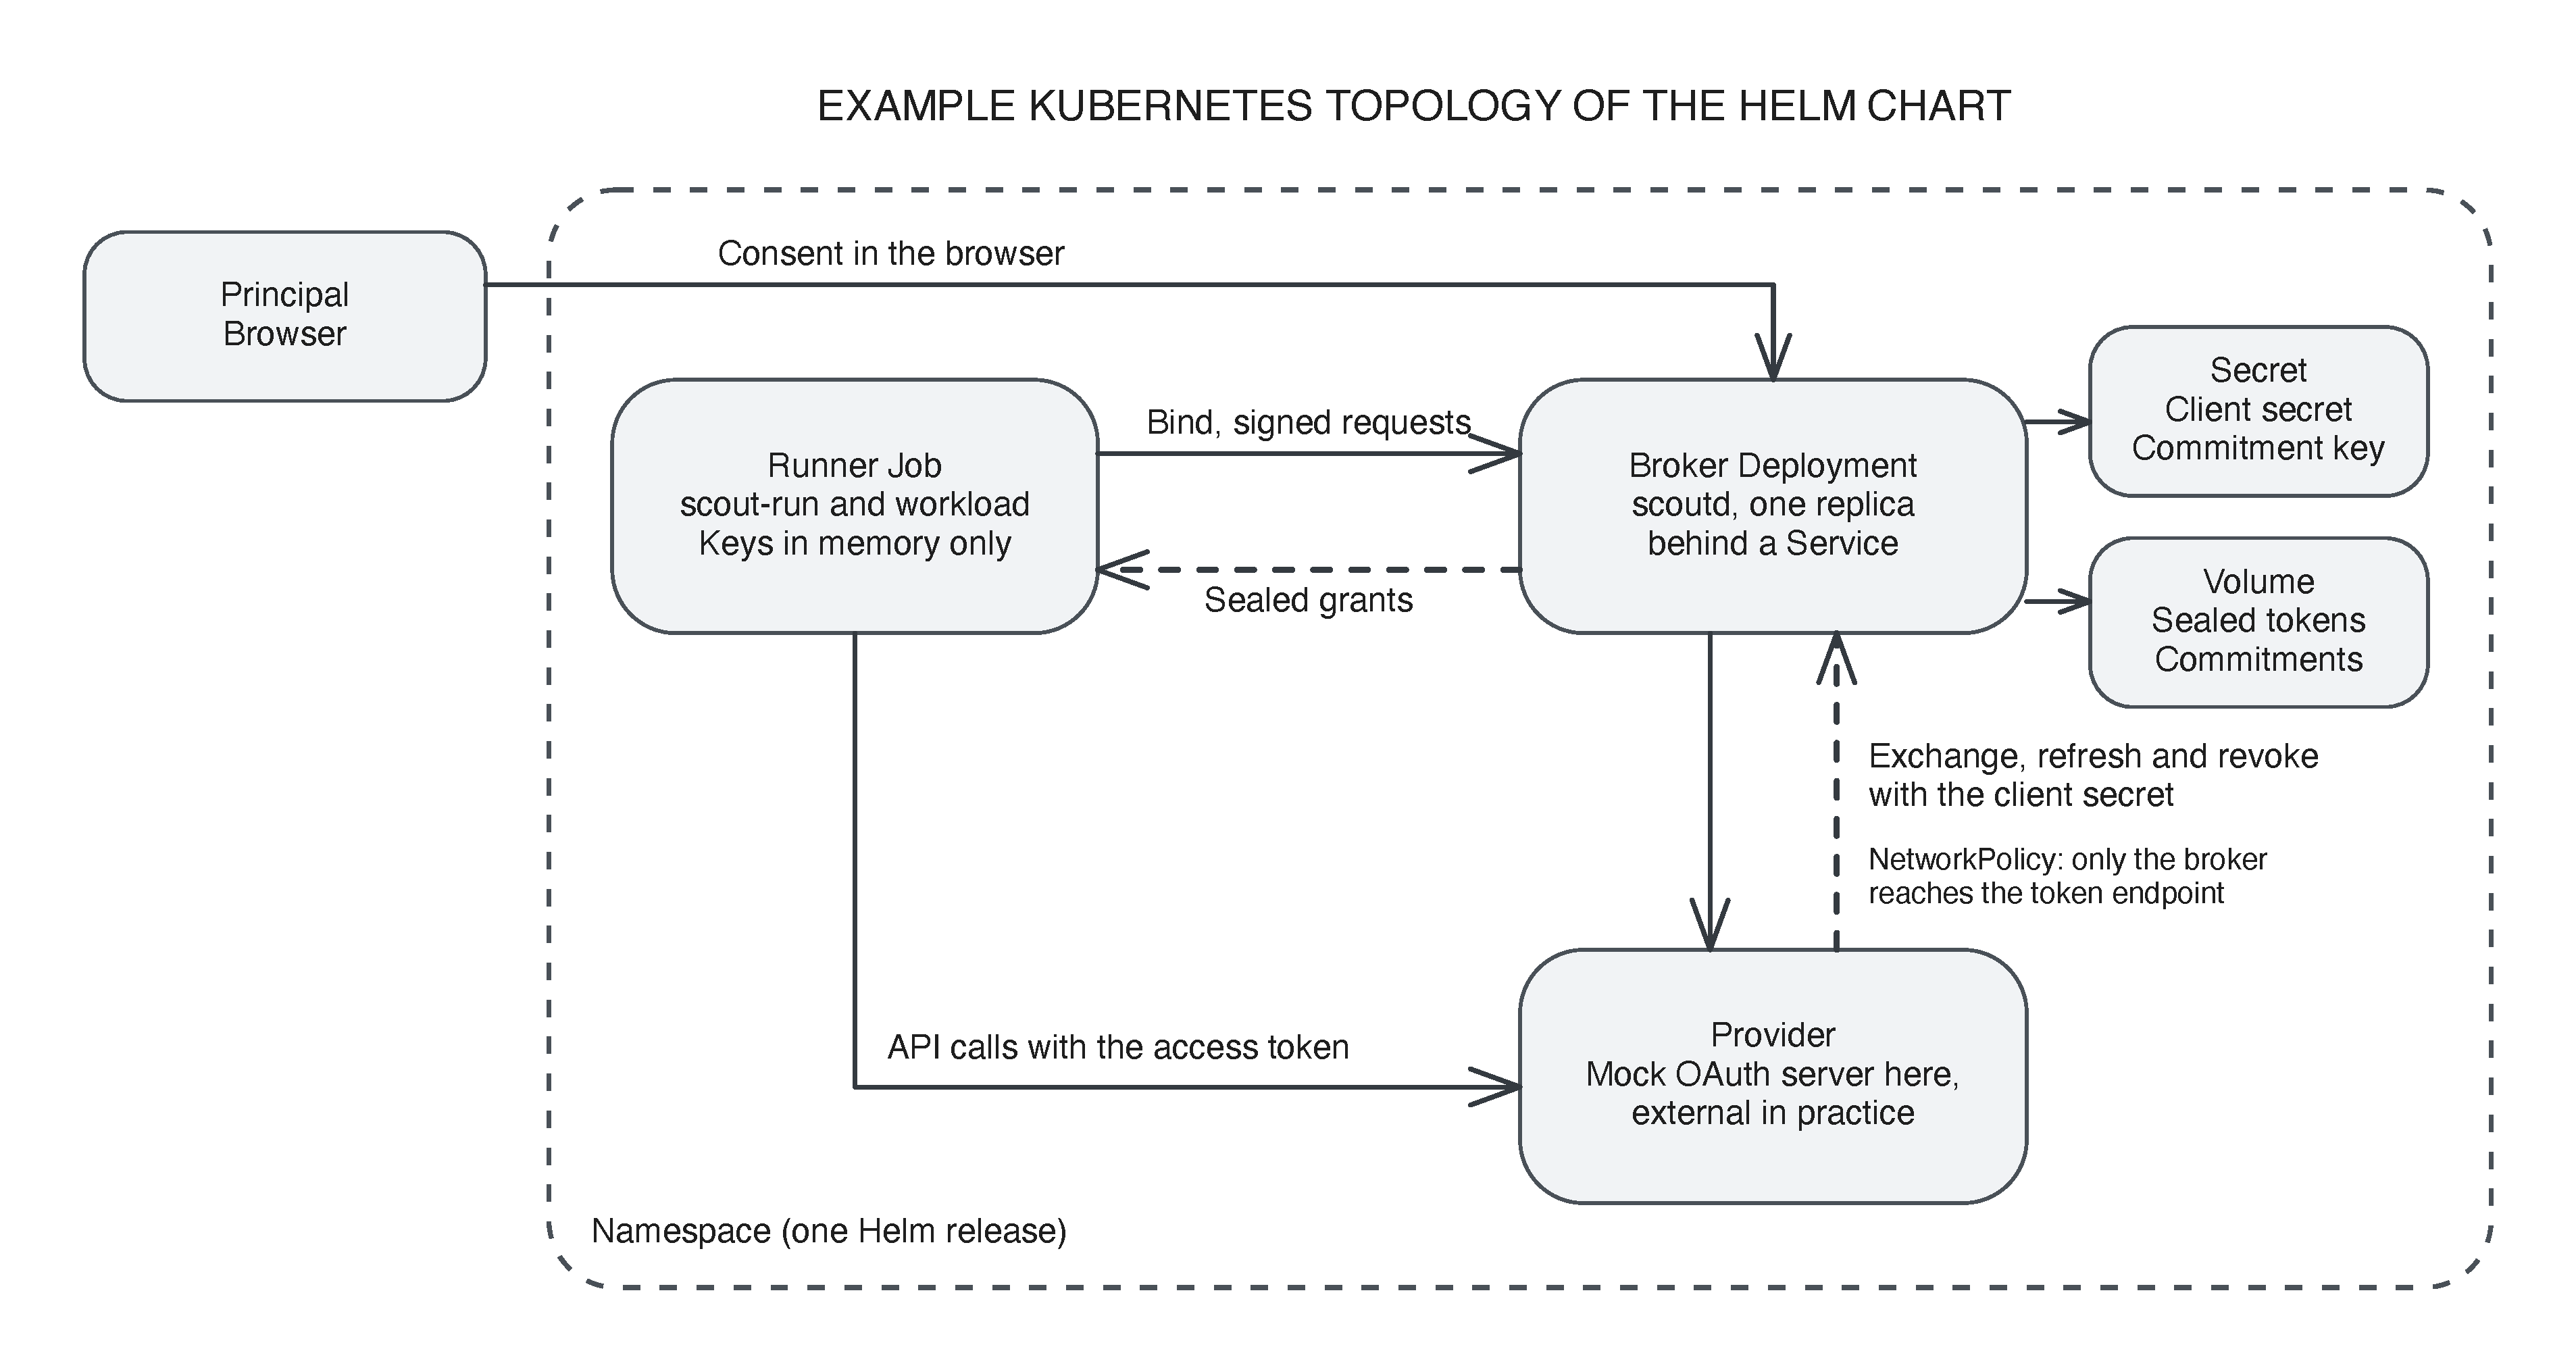
\includegraphics[width=0.9\textwidth]{fig/fig7.pdf}
\caption{Example deployment of the reference implementation. The runner holds its keys in memory; the broker reads the client secret and commitment key from a Secret and keeps only sealed tokens and commitments on its volume; a NetworkPolicy lets only the broker reach the provider's token endpoint.}
\label{fig:k8s}
\end{figure}

\paragraph{A pure protocol core.} Every protocol decision is taken by one crate that has no dependencies and performs no I/O, reads no clock, and uses no randomness or cryptography. It contains the session reducer, the delivery record, the renewal control record and the teardown ordering as total functions from a state and an event to a new state or a rejection. Tokens, commitments, ciphertexts and operation identifiers appear in it only as opaque values. The surrounding crates do the cryptography and storage and translate their results into those values, for example by comparing a recomputed commitment in constant time and passing the outcome in. No decision is duplicated outside the core, so a property proved of the core constrains what the service can do.

\paragraph{Verification of the code with Kani.} Kani~\cite{kani} is a bit-precise model checker for Rust. We state the properties of Table~\ref{tab:smt} for the core and prove them inductively on the compiled code: a harness takes an arbitrary state that satisfies the invariant, applies one arbitrary event with arbitrary parameters, and asserts the invariant on the result, so the conclusion holds for any number of steps. Properties that refer to history, such as the number of provider exchanges for a generation, use ghost fields that exist only in verification builds. Fourteen harnesses cover the session properties F1--F4, the delivery properties D1--D2, the renewal properties S1--S5 and the teardown properties T1--T6; all are verified. Four deliberately broken variants of the core (no principal lock, a new request receives a new response, no commitment check, revocation of any submitted token) are compiled behind a feature flag, and Kani reports a failure for each.

\paragraph{Tests of the whole service.} Kani covers the core only. The rest is tested. An exhaustive search drives the real renewal code, with the real store and an injected clock, through every sequence of begin, exchange, commit, crash, close and lapse for generations zero to two, and checks S1--S5 on each of the 266 reachable states; with the broken core it fails. End-to-end tests run broker and provider in process and cover a lost reply (the retry receives the identical ciphertext and the provider records exactly one refresh), a competing operation, a provider reply lost before commit (no later retry reaches the provider and fresh consent is required), a token of another session (rejected with no provider call), a dump of the store (no token plaintext), closure, revocation of an undelivered token, a broker restart, and supervision of the workload's process group. Continuous integration runs these, the adversarial tests and isolated attack run described below, the proofs of Section~\ref{sec:eval}, the Kani proofs, a full session under Docker Compose, and an installation of the Helm chart on a Kubernetes cluster in which the example job must complete.

\paragraph{Review of the code around the core.} After the first version of this paper was archived, the code outside the core was reviewed adversarially and then tested further. The review found no defect in the broker's protocol path, and confirmed by reading that the commitment check precedes every use of the client authentication, that a crash between the provider call and the commit cannot lead to a second provider call, and that store updates are atomic. It did find defects elsewhere, and the first version of this section claimed more than the code delivered. The most serious was in the runner: on a termination signal or a panic it exited without revoking or finalizing, and the workload survived with its access token. The runner now handles the signals, stops the whole process group, and revokes and finalizes on every exit path that it can observe. The others were: the runner accepted a sealed reply for any grant and generation named in the reply itself; a renewal whose reply was lost during a long broker outage was abandoned although it was still replayable; the hand-written HTTP server read header lines without a bound and had no total request deadline or connection limit; a consent callback could delete the closed marker left by finalization; low-order public keys were accepted at binding; and the store file was neither private nor locked. Each was fixed together with a test that fails on the old code. The tests added at the same time send thirty-eight thousand generated malformed requests to the server, run thirty-two concurrent renewals per generation, kill and restart the broker at each critical point, and scan all output and the store for secrets. Kani additionally proves that one small parsing function of the transport layer cannot panic for bounded inputs.

\paragraph{An isolated attack run.} A further scenario runs in containers on networks without outbound access, with read-only filesystems and no capabilities. The attacker holds a legitimate session of its own and a refresh token deliberately leaked by a victim session. It attempts to read the victim's grants, to bind its key to the victim's session without the session secret, to renew with the stolen token through its own session, to renew the victim's session, to replay one of its own renewals under another operation identifier, to revoke a token that was not delivered to it, to reach the provider's back channel, to redeem the stolen token at the provider without the client authentication, and to fetch after finalization. All are refused, and the victim's session completes. This run is part of continuous integration.

\paragraph{What writing it showed.} Implementing from the paper exposed one point the text had left open: which receipt a retry presents after the generation has advanced. The implementation accepts, for the committing operation only, the receipt of the generation that the saved reply replaced; the exhaustive search found the first attempt at this rule wrong. It also showed that a NetworkPolicy cannot separate a provider's token endpoint from its other routes on one port, so the example serves the back channel on a port of its own.

\section{Discussion and Limitations}
\label{sec:limits}
\begin{itemize}
\item \textbf{Not a lifetime reduction.} Local expiry, cancellation or deletion does not invalidate provider tokens by itself. Cancellation cannot recall a ciphertext already released or a provider request already authorized; revalidation just before dispatch narrows but cannot close that window because the provider is an independent system.
\item \textbf{Provider-dependent.} Split custody applies where the provider requires confidential-client authentication. With public-client refresh, session gating and sealed delivery still apply but the split of client authentication does not.
\item \textbf{Rollback.} The safety properties assume the authoritative control state is not replaced by an older authentic snapshot; deployments without that guarantee need an independently trusted monotonic state to detect rollback.
\item \textbf{Ambiguity is conservative.} After a broker crash between provider call and commit, SCOUT fails closed and requires reconciliation or new consent, trading availability for not repeating a possibly-consumed refresh token. Loss of the runner key likewise requires new consent.
\item \textbf{Runner compromise.} A runner that is compromised during its session has the tokens it holds; the supervisor design reduces but does not remove trust in the host and supervisor.
\end{itemize}

\section{Related Work}
\paragraph{Runner-sealed job credentials.} The GitHub Actions runner encrypts a job's OAuth token to a runner-held key and revokes it at job end~\cite{ghrunner}. It delivers a token minted for the job; it does not renew a user's rotating refresh token under split custody.

\paragraph{Backend-held client credentials.} The browser-based-apps guidance has a confidential backend refresh on behalf of a user session~\cite{bff}, and the Spotify token-swap pattern has a mobile app send its refresh token to a server that holds the client secret, suggesting the token be returned encrypted~\cite{spotify}. Both keep the secret off the device. Neither checks the presented token against an approved lineage before using the secret, and neither replays a lost rotating reply.

\paragraph{Token vaults and agent credential brokers.} Auth0 Token Vault keeps provider tokens at the identity service~\cite{auth0}. Posta's series on credential injection for agents describes envelope-encrypted vaults with owner-bound associated data~\cite{agentgateway} and separates a refresher that holds refresh tokens and client secrets from a controller that stores access tokens~\cite{posta}; an IETF individual draft proposes a credential broker for agents with DPoP-bound short-lived tokens~\cite{hartman}. These place refresh material in a component that can use it.

\paragraph{Sender-constrained tokens and client attestation.} DPoP~\cite{rfc9449} and attestation-based client authentication~\cite{attest} bind tokens or client instances to keys at the provider, and the OAuth security best current practice recommends sender-constraining or rotating refresh tokens~\cite{rfc9700}. They need provider support. SCOUT's implemented path works against an unmodified confidential-client provider, and Section~\ref{sec:assertion} shows where provider support would strengthen it.

\paragraph{Lost replies and idempotency.} Idempotency keys save and replay a first response~\cite{stripe}. The Hydra issue on refresh-token rotation records why a hash-only token store cannot do this and what the grace-period workaround costs~\cite{hydra1831}. Sequence-numbered join state that locks on a stale value appears in Teleport's bound-keypair joining~\cite{teleport}, and Vault response wrapping gives single-use sealed delivery~\cite{vaultwrap}.

\paragraph{Credential-injecting proxies and attenuation.} Sandboxed coding agents commonly keep the real token outside the sandbox and attach it in a proxy after checking the operation~\cite{anthropicsandbox}; Fly.io's tokenizer seals a secret together with host restrictions~\cite{tokenizer}. Delegation graphs with scope intersection appear in the patent literature~\cite{us12671588}. Our supervisor follows this line; what it adds is the interaction with renewal, where concurrent children are served by one reserved rotation of the shared family and each operation is re-evaluated after replacement.

\paragraph{Capabilities, token exchange and workload identity.} Macaroons~\cite{macaroons} let the holder of a bearer credential attenuate it by appending caveats that the target service verifies; this gives decentralized narrowing of authority, but only at a service that issues and understands macaroons. OAuth token exchange~\cite{rfc8693} lets a client trade one token for a narrower or delegated one at the authorization server, again given provider support. SPIFFE~\cite{spiffe} gives a workload a verifiable identity of its own; it answers which workload is calling, not which human approved what. SCOUT's supervisor reaches a similar narrowing for a provider that offers none of these, by keeping the broad token behind a mediation boundary, and its renewal protocol is orthogonal to all three: each of them still needs some party to hold whatever renews the underlying credential.

\paragraph{Positioning.} Each ingredient has precedent: sealing to a recipient key~\cite{rfc9180}, keeping the client secret at a backend, keyed token digests, idempotent replay, compare-and-swap on a version counter. To our knowledge the combination has not been described: storage the broker cannot decrypt, replay of a lost single-use refresh reply from that storage, and a lineage check that precedes any use of the client authentication.

\section{Conclusion}
Credential renewal for unattended agents need not collect a decryptable refresh token at a broker or ship client secrets into every runner. Splitting custody, gating renewal on a live key-pinned session, binding renewal to the approved token lineage, recording renewal as a recoverable generation, attempting revocation before deletion, and mediating agent operations behind an isolated supervisor together give a design whose residual risk is bounded by stated assumptions and by provider behaviour. The broker state this needs contains no usable secret: a keyed commitment, a generation counter with one reserved operation, and ciphertext only the runner can open. The same state gives a principled answer to ambiguity: do not retry; ask the human again. The core invariants are machine-checked for unbounded executions, the secrecy and binding properties are proved against an active attacker, and we hope the explicit assumptions, failure branches and broken variants are useful to others building similar brokers.

\appendix
\section*{Reproducibility note}
Everything is public at \url{https://github.com/Algiras/scout-proofs} and archived with this paper at \url{https://doi.org/10.5281/zenodo.24568572}. The paper, proofs and diagrams are licensed under CC BY 4.0 and the code under Apache License 2.0. This is version 2; it differs from version 1 in the review and hardening of the reference implementation described in Section~\ref{sec:impl}, and makes no change to the protocol or the proofs. \texttt{proofs/scout\_smt.py} generates every SMT-LIB obligation and bounded-model-checking query, runs Z3 (4.15.4) and prints the tables of Section~\ref{sec:eval}; the obligations are also stored as \texttt{.smt2} files so they can be checked with another solver. \texttt{proofs/export.py} translates the same models to Lean~4 and TLA\textsuperscript{+} and runs the Lean kernel (4.36.0) on the 63 theorems and TLC (TLA\textsuperscript{+} tools 1.8.0) on the 32 modules. \texttt{proofs/symbolic/} holds three scripts that generate and run the seventeen ProVerif models (2.05) and compare each result with its expected value. \texttt{impl/} is the reference implementation; \texttt{cargo test} runs its tests, \texttt{cargo kani} in \texttt{impl/scout-core} runs the code-level proofs (Kani 0.68.0), and \texttt{impl/isolated/docker-compose.yml} is the isolated attack run. \texttt{deploy/helm/scout} is the Helm chart. Each script exits with success only if every proof passes and every broken variant is caught, and the repository's continuous integration runs all of them.

\begin{thebibliography}{99}\small
\bibitem{rfc9700} T. Lodderstedt, J. Bradley, A. Labunets, D. Fett. \emph{Best Current Practice for OAuth 2.0 Security}. RFC 9700 (BCP 240), January 2025. \url{https://www.rfc-editor.org/info/rfc9700}
\bibitem{rfc9449} D. Fett, B. Campbell, J. Bradley, T. Lodderstedt, M. Jones, D. Waite. \emph{OAuth 2.0 Demonstrating Proof of Possession (DPoP)}. RFC 9449, September 2023. \url{https://www.rfc-editor.org/info/rfc9449}
\bibitem{rfc9180} R. Barnes, K. Bhargavan, B. Lipp, C. Wood. \emph{Hybrid Public Key Encryption}. RFC 9180, February 2022. \url{https://www.rfc-editor.org/info/rfc9180}
\bibitem{rfc7523} M. Jones, B. Campbell, C. Mortimore. \emph{JSON Web Token (JWT) Profile for OAuth 2.0 Client Authentication and Authorization Grants}. RFC 7523, May 2015. \url{https://www.rfc-editor.org/info/rfc7523}
\bibitem{rfc7591} J. Richer (ed.), M. Jones, J. Bradley, M. Machulak, P. Hunt. \emph{OAuth 2.0 Dynamic Client Registration Protocol}. RFC 7591, July 2015. \url{https://www.rfc-editor.org/info/rfc7591}
\bibitem{rfc7009} T. Lodderstedt (ed.), S. Dronia, M. Scurtescu. \emph{OAuth 2.0 Token Revocation}. RFC 7009, August 2013. \url{https://www.rfc-editor.org/info/rfc7009}
\bibitem{bff} A. Parecki, P. De Ryck, D. Waite. \emph{OAuth 2.0 for Browser-Based Applications}. RFC 10017 (BCP 212), August 2026; previously draft-ietf-oauth-browser-based-apps. \url{https://datatracker.ietf.org/doc/draft-ietf-oauth-browser-based-apps/}
\bibitem{attest} T. Looker, P. Bastian, C. Bormann. \emph{OAuth 2.0 Attestation-Based Client Authentication}. IETF Internet-Draft draft-ietf-oauth-attestation-based-client-auth-12, October 2026. Work in progress. \url{https://datatracker.ietf.org/doc/draft-ietf-oauth-attestation-based-client-auth/}
\bibitem{hartman} K. G. Hartman. \emph{Credential Broker for Agents (CB4A)}. IETF individual Internet-Draft draft-hartman-credential-broker-4-agents-00, March 2026 (expired). \url{https://datatracker.ietf.org/doc/draft-hartman-credential-broker-4-agents/}
\bibitem{ghrunner} GitHub. \emph{Runner Authentication and Authorization}. Design document in the \texttt{actions/runner} repository. \url{https://github.com/actions/runner/blob/main/docs/design/auth.md}
\bibitem{ghrefresh} GitHub Docs. \emph{Refreshing user access tokens}. \url{https://docs.github.com/en/apps/creating-github-apps/authenticating-with-a-github-app/refreshing-user-access-tokens}
\bibitem{spotify} Spotify for Developers. \emph{Token Swap and Refresh}. \url{https://developer.spotify.com/documentation/ios/guides/token-swap-and-refresh}
\bibitem{stripe} Stripe API documentation. \emph{Idempotent requests}. \url{https://docs.stripe.com/api/idempotent_requests}
\bibitem{hydra1831} Ory Hydra. \emph{Refresh tokens need a grace period to deal with network errors and similar issues}. Issue \#1831, April 2020, \url{https://github.com/ory/hydra/issues/1831}; and Ory documentation, \emph{Graceful token refresh}, \url{https://www.ory.com/docs/hydra/guides/graceful-token-refresh}
\bibitem{teleport} Teleport documentation. \emph{Joining Services with Bound Keypair}. \url{https://goteleport.com/docs/installation/agents/bound-keypair/}
\bibitem{vaultwrap} HashiCorp Vault documentation. \emph{Response wrapping}. \url{https://developer.hashicorp.com/vault/docs/concepts/response-wrapping}
\bibitem{auth0} Auth0 documentation. \emph{Token Vault}. \url{https://auth0.com/docs/secure/call-apis-on-users-behalf/token-vault}
\bibitem{posta} C. Posta. \emph{Credential Injection Patterns for AI Agents: Part 2.5, Where KMS Grants Stop Scaling}. agentgateway blog, October 2026. \url{https://agentgateway.dev/blog/2026-10-20-credential-brokering-mode-3-at-scale/}
\bibitem{agentgateway} C. Posta. \emph{Credential Injection Patterns for AI Agents: Part 2, Securing the Vault}. agentgateway blog, August 2026. \url{https://agentgateway.dev/blog/2026-08-03-protecting-token-vault-kms-credential-injection/}
\bibitem{anthropicsandbox} Anthropic. \emph{Beyond permission prompts: making Claude Code more secure and autonomous}. Engineering blog, October 2025. \url{https://www.anthropic.com/engineering/claude-code-sandboxing}
\bibitem{tokenizer} Fly.io. \emph{Tokenized Tokens}, \url{https://fly.io/blog/tokenized-tokens/}; and the \texttt{superfly/tokenizer} repository, \url{https://github.com/superfly/tokenizer}
\bibitem{us12671588} Y. B. Lee. \emph{Identity-bound delegated authorization, connector mediation, and offline-verifiable receipt lineage for agentic systems}. US Patent 12,671,588 B1, June 2026. \url{https://patents.google.com/patent/US12671588B1/en}
\bibitem{macaroons} A. Birgisson, J. G. Politz, {\'U}. Erlingsson, A. Taly, M. Vrable, M. Lentczner. Macaroons: Cookies with contextual caveats for decentralized authorization in the cloud. In \emph{NDSS}, 2014. \url{https://doi.org/10.14722/ndss.2014.23212}
\bibitem{rfc8693} M. Jones, A. Nadalin, B. Campbell (ed.), J. Bradley, C. Mortimore. \emph{OAuth 2.0 Token Exchange}. RFC 8693, January 2020. \url{https://www.rfc-editor.org/info/rfc8693}
\bibitem{spiffe} SPIFFE. \emph{SPIFFE overview}. \url{https://spiffe.io/docs/latest/spiffe-about/overview/}
\bibitem{proverif} B. Blanchet. Modeling and verifying security protocols with the applied pi calculus and ProVerif. \emph{Foundations and Trends in Privacy and Security}, 1(1--2):1--135, 2016. \url{https://doi.org/10.1561/3300000004}
\bibitem{lean4} L. de Moura, S. Ullrich. The Lean 4 theorem prover and programming language. In \emph{CADE-28}, LNCS 12699, pp.~625--635, 2021. \url{https://doi.org/10.1007/978-3-030-79876-5_37}
\bibitem{tla} L. Lamport. \emph{Specifying Systems: The TLA+ Language and Tools for Hardware and Software Engineers}. Addison-Wesley, 2002. \url{https://lamport.azurewebsites.net/tla/book.html}
\bibitem{kani} A. VanHattum, D. Schwartz-Narbonne, N. Chong, A. Sampson. Verifying dynamic trait objects in Rust. In \emph{ICSE-SEIP}, 2022. \url{https://doi.org/10.1145/3510457.3513031}
\bibitem{z3} L. de Moura, N. Bj{\o}rner. Z3: An efficient SMT solver. In \emph{TACAS 2008}, LNCS 4963, pp.~337--340. \url{https://doi.org/10.1007/978-3-540-78800-3_24}

\smallskip\noindent Web pages were accessed in November 2026.
\end{thebibliography}

\end{document}
